\documentclass[a4paper,12pt]{article}

% ================================================== DATOS ==================================================

% Información de la materia
\newcommand{\codMateria}{TA138}
\newcommand{\nombreMateria}{Taller de Diseño de}
\newcommand{\cuatrimestre}{1.\textsuperscript{er} Cuatrimestre}

% Información del TP
\newcommand{\TpTitulo}{Proyecto Integrador -- Checkpoint 2}
\newcommand{\fecha}{\today}
\newcommand{\group}{Grupo 5}

% Información de alumnos
\newcommand{\nombreA}{Lautaro García Vitale}
\newcommand{\padronA}{110028}
\newcommand{\emailA}{lagarciav@fi.uba.ar}

\newcommand{\nombreB}{Santiago Manuel Cabrera}
\newcommand{\padronB}{110445}
\newcommand{\emailB}{smcabrera@fi.uba.ar}

\newcommand{\nombreC}{Francisco Javier Moya}
\newcommand{\padronC}{109899}
\newcommand{\emailC}{fjmoya@fi.uba.ar}

% ================================================== PAQUETES =================================================

% Codificación y lenguaje
\usepackage[utf8]{inputenc}
\usepackage[ddmmyy]{datetime}
\usepackage[language=spanish]{lipsum}
\usepackage[spanish]{datetime2}
\usepackage[T1]{fontenc}
\usepackage[spanish,es-nodecimaldot]{babel}
\usepackage[a4paper,margin=2.5cm]{geometry}
\usepackage{amsmath,amssymb,amsthm,mathtools}
\usepackage{bm}
\usepackage{physics}
\usepackage{setspace}
\usepackage{hyperref}
\usepackage{enumitem}

% Márgenes y página
\usepackage{geometry}
\usepackage{fancyhdr}
\usepackage{emptypage}
\usepackage{parskip}

% Encabezado personalizado
\pagestyle{fancy}
\fancyhf{}
\rhead{\group}
\lhead{\TpTitulo}
\cfoot{\thepage}

% Tipografía matemática
\usepackage{mathtools}
\usepackage{amssymb}
\usepackage{amsfonts}
\usepackage{amsthm}
\usepackage{yhmath}
\usepackage{dsfont}
\usepackage{esdiff}
\usepackage{xfrac}
\usepackage{siunitx}
\sisetup{per-mode=reciprocal, separate-uncertainty=true}

% Gráficos y tablas
\usepackage{graphicx}
\usepackage{float}
\usepackage{booktabs}
\usepackage{caption}
\usepackage{subcaption}
\usepackage{multirow}
\usepackage{adjustbox}

% TikZ y gráficos avanzados
\usepackage{pgfplots}
\pgfplotsset{compat=1.18}
\usepackage{tikz}

% Código fuente y resaltado
\usepackage{minted}
\usepackage{tcolorbox}
\definecolor{codebg}{rgb}{0.95,0.95,0.95}  % Color de fondo del código
\usemintedstyle{friendly}                  % Estilo del resaltado de sintaxis
\setminted{
    linenos=true,                          % Numeración de líneas
    bgcolor=codebg,                        % Color de fondo del código
    fontsize=\footnotesize,                % Tamaño de la fuente
    frame=lines,                           % Estilo del marco
    framesep=2mm,                          % Separación del marco
    baselinestretch=1.2,                   % Espaciado entre líneas
    breaklines=true,                       % Romper líneas largas automáticamente
    encoding=utf8,                         % Codificación del archivo
    tabsize=4,                             % Tamaño de la tabulación
}

% Misceláneo
\usepackage{anyfontsize}
\usepackage{xcolor}
\usepackage{url}
\usepackage{comment}
\usepackage{multicol}
\usepackage[numbers,square]{natbib}

% Estilo de bibliografía
\bibliographystyle{IEEEtran}


% ==============================================================================================================
% ==============================================================================================================


\begin{document}

% ================================================== CARÁTULA ==================================================

\pagenumbering{arabic} % Comienza la numeración

\vspace{-1 cm} % La primera hoja tiene que tener menos espaciado

\begin{center}
  \begin{minipage}{0.8 cm}
    
\includegraphics[width=\linewidth]{img/fiuba.png}
  \end{minipage}
  \begin{minipage}{\widthof{\large{\textsc{Universidad de Buenos Aires}}}}
    \centering
    \large{\textsc{Universidad de Buenos Aires}}\\
    \large{\textsc{Facultad de Ingeniería}}\\
    \small{Año 2026 -- \cuatrimestre}
  \end{minipage}
\end{center}
\vspace{10mm}
\begin{center}
  \huge{\underline{\textsc{\nombreMateria}}} \\
  \huge{\underline{\textsc{Circuitos Electrónicos}}} \\
  \vspace{7 pt}
  \Large{\TpTitulo \\}
  \vspace{3mm}
  \large{\group}
\end{center}

\newcommand{\anchopadron}{\widthof{000 000}}
\begin{center}
  \begin{tabular}{l l l}
    \nombreA & \parbox{\anchopadron}{\raggedleft \padronA} & \emailA \\
    \nombreB & \parbox{\anchopadron}{\raggedleft \padronB} & \emailB \\
    \nombreC & \parbox{\anchopadron}{\raggedleft \padronC} & \emailC 
  \end{tabular}
\end{center}
\vspace{8mm}

\begin{center}
\renewcommand{\arraystretch}{1.3}
\begin{tabular}{@{}r p{0.62\textwidth}@{}}
\textbf{Tutor:} & Federico Gabriel D'Angiolo. \\ 
\textbf{Docentes:} & Julio Guillermo Zola, Marcelo Adrián Bruno, Sergio Quinteros y Juan Guido Salaya.
\end{tabular}
\end{center}

\vspace{2em}
\thispagestyle{empty}

\begin{abstract}
El presente informe detalla el desarrollo del segundo \textit{checkpoint} del proyecto integrador, enfocado en asegurar la estabilidad dinámica y la integridad física del regulador lineal LDO diseñado previamente. 

En primer lugar, se realiza un análisis exhaustivo de la respuesta en frecuencia mediante el estudio de los diagramas de Bode para los lazos de realimentación de tensión y corriente. Se evalúan los márgenes de fase y de ganancia para determinar la estabilidad del sistema y, en caso de ser necesario, se proponen e implementan redes de compensación de frecuencia que garanticen un comportamiento robusto frente a transitorios. 

Posteriormente, se aborda el análisis térmico del regulador, considerando las condiciones críticas de operación y la potencia disipada por el transistor de paso. Este estudio permite dimensionar y seleccionar el disipador de calor adecuado para mantener las temperaturas de juntura dentro de los límites de seguridad. 

Finalmente, se presenta el diseño definitivo del circuito impreso (PCB) en entorno CAD, optimizando el ruteo de las pistas de potencia y señal, así como la disposición de los componentes para facilitar la posterior implementación física y validación experimental del sistema.
\end{abstract}

\newpage

\tableofcontents

\newpage

\section{Introducción}
El diseño de una fuente de alimentación para entornos industriales y automotrices exige no solo precisión en los niveles de tensión continua, sino también robustez frente a variaciones dinámicas y condiciones térmicas adversas. En el primer checkpoint de este proyecto, se estableció la topología del regulador lineal LDO, basada en un par diferencial con carga activa y una etapa de potencia cuasi-darlington, integrando además una protección de tipo \textit{foldback}.

Si bien el diseño estático garantiza una salida de $\SI{5}{\volt}$ y una limitación de corriente adecuada, el comportamiento del sistema en el dominio de la frecuencia y su gestión térmica son fundamentales para su viabilidad física. Un regulador con alta ganancia de lazo, como el propuesto, corre el riesgo de volverse inestable y oscilar si los márgenes de fase no son suficientes ante la presencia de múltiples polos en la función de transferencia.

En este contexto, el presente informe aborda la segunda etapa del diseño circuital e integración. Los objetivos principales son:
\begin{itemize}
    \item Analizar la estabilidad de los lazos de control de tensión y corriente mediante diagramas de Bode, aplicando técnicas de compensación de frecuencia si el margen de fase resulta insuficiente.
    \item Evaluar el comportamiento térmico del transistor de paso TIP32, calculando la resistencia térmica necesaria para evacuar el calor generado y seleccionando un disipador comercial compatible.
    \item Documentar el diseño del PCB, considerando criterios de integridad de señal y manejo de altas corrientes para la posterior fabricación del prototipo.
\end{itemize}

\section{Compensación}

\subsection{Lazo de tensión}

En esta sección se analizará la estabilidad del lazo de tensión en \texttt{LTSpice}, para lo cual se utilizó el circuito de la \autoref{fig:circuito LT}.

\begin{figure}[H]
    \centering
    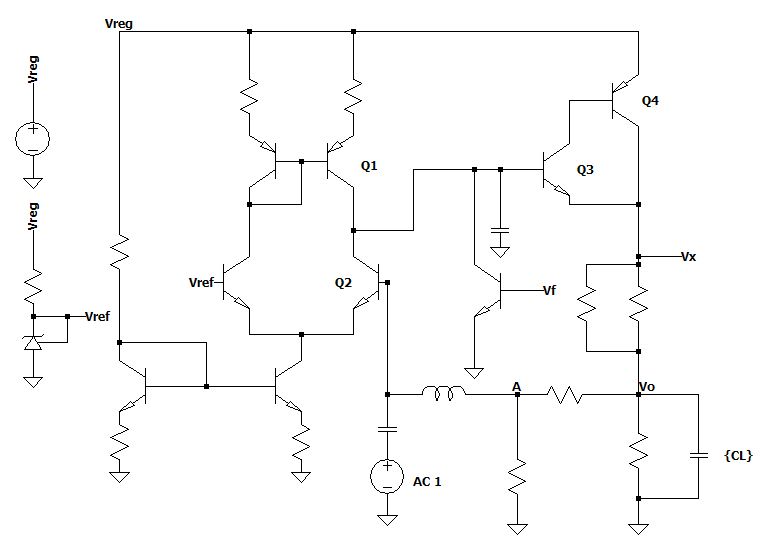
\includegraphics[width=0.9\linewidth]{img/Lazo de tensión/Circuito LT.png}
    \caption{Circuito utilizado para medir el lazo de tensión}
    \label{fig:circuito LT}
\end{figure}

En el mismo, la fuente de tensión \texttt{AC 1} funciona como la entrada a una de las terminales del par diferencial y se mide la salida del realimentador f (nodo A), obteniendo así la transferencia $L = a\cdot f$. El capacitor unido a la base de Q3 es el capacitor de compensación, que en principio es de 0 F.

Como puede verse en las directivas, la capacidad $C_L$ puede tomar 2 valores, \SI{1}{\micro \farad} y \SI{15}{\micro \farad}. Además, la carga puede variar entre \SI{3,4}{\ohm} y \SI{50}{\ohm}, por lo que se tienen 4 circuitos distintos para compensar. Para hacer la tarea más simple se optó por compensar el circuito con el peor margen de fase, lo que compensaría a todos a la vez. Luego de un breve análisis de obtuvo que el peor caso se da para la combinación $R_L = 50 \Omega$ y $C_L = \SI{1}{\micro \farad}$, cuyo diagrama de Bode se muestra el la \autoref{fig:LT sin compensar}

\begin{figure}[H]
    \centering
    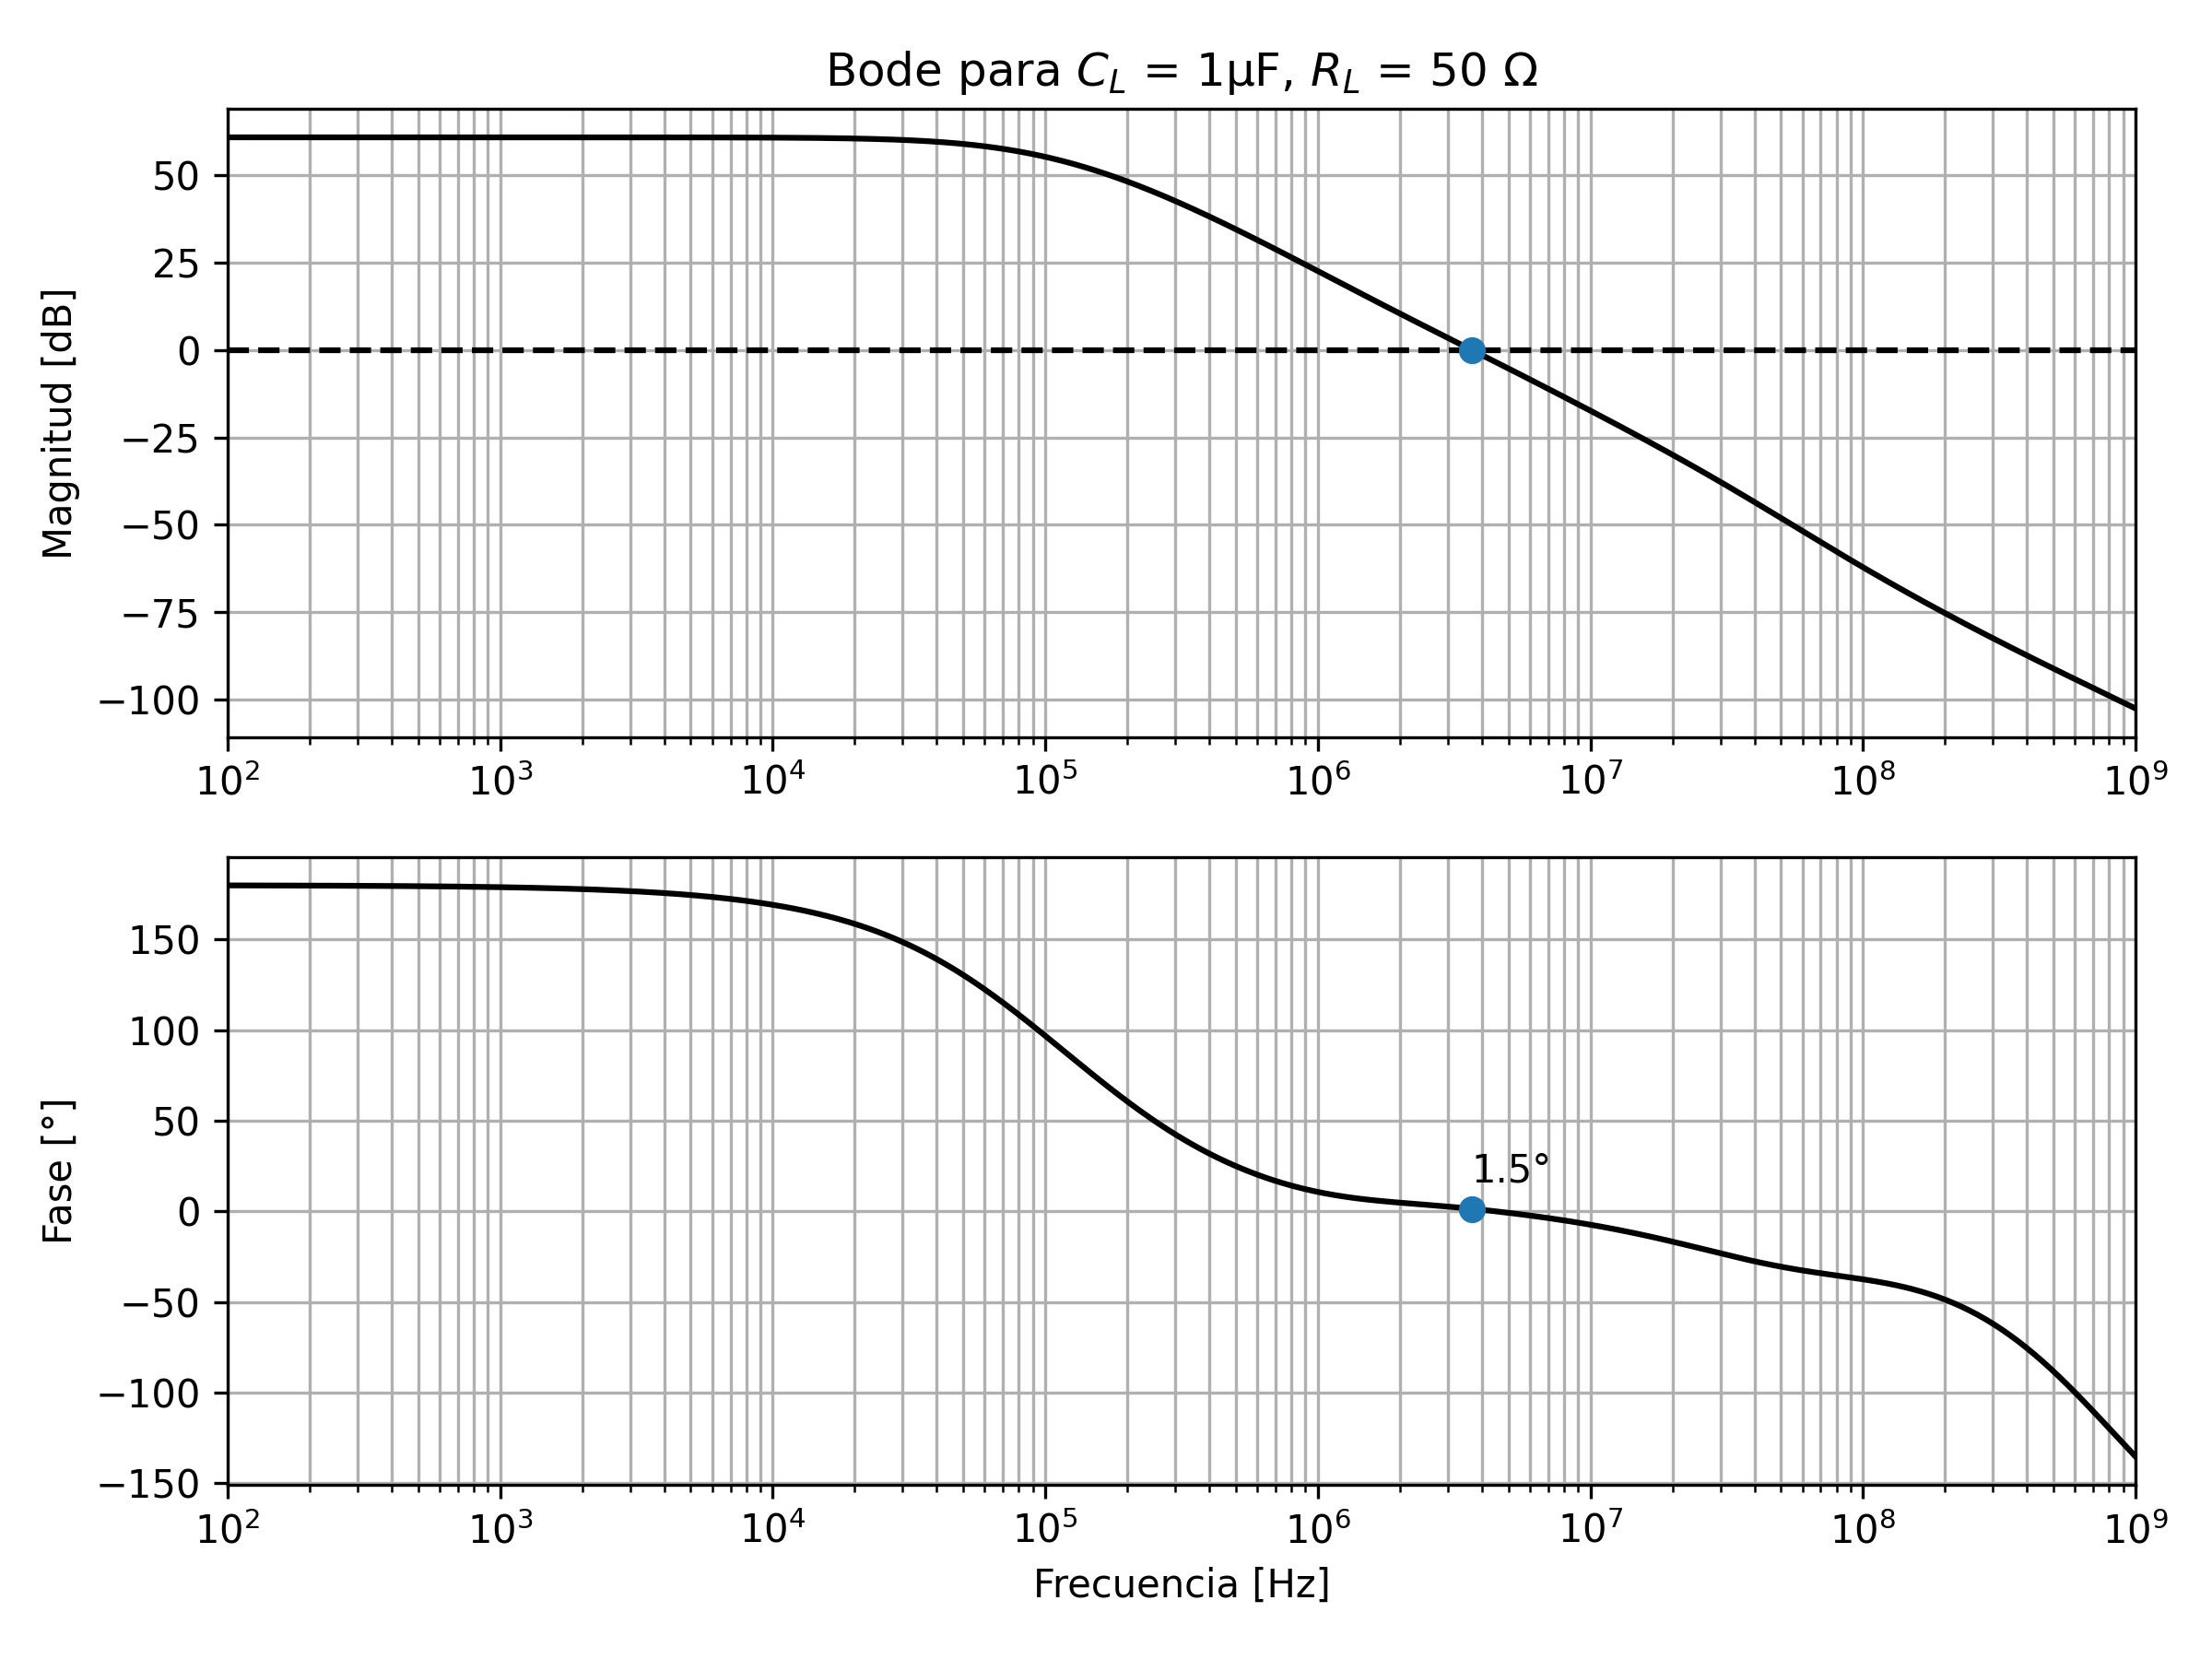
\includegraphics[width=0.9\linewidth]{img/Lazo de tensión/LT sin compensar.png}
    \caption{Lazo de tensión sin compensar para $R_L = 50 \Omega$ y $C_L = \SI{1}{\micro \farad}$}
    \label{fig:LT sin compensar}
\end{figure}

Se observa que el margen de fase es muy chico, por lo que el circuito está al borde de la inestabilidad. Por otro lado, se observa que el polo dominante está a aproximadamente \SI{100}{\kilo \hertz}. Analizando el circuito, puede intuirse que el polo dominante se debe al nodo de salida del par diferencial, ya que este es el nodo con más capacitores unidos. Habrá entonces una capacidad y una resistencia equivalentes entre el nodo y tierra, lo que implicaría un valor para el polo dominante de $p = \frac{1}{2\pi R_N C_N}$. Por lo tanto, puede agregarse un capacitor entre el nodo y tierra, el cual se sumaría al valor de la capacidad ya presente en el nodo y reduciría la frecuencia del polo dominante. 

Para estimar un valor para el capacitor de compensación, puede calcularse de forma aproximada la capacidad equivalente del nodo $C_N$ usando la técnica de reflexión de Miller. 

\begin{equation}
    C_N = C_{\mu1} + C_{\mu2} + C_{\mu3}\cdot (1 + g_{m3} \, r_{\pi4}) = \SI{22}{\pico \farad}
\end{equation}

En esta ecuación los valores de la resistencia, transconductancia y capacidades se obtuvieron de una simulación \texttt{.op} de \texttt{LTSpice}. Cabe aclarar que este resultado es solo una aproximación, ya que se hicieron varias simplificaciones, como que la ganancia base-colector de Q3 era 1 y que en frecuencia el capacitor $C_L$ es un cortocircuito.

En cualquier caso, se necesita disminuir el valor del polo dominante en por lo menos 3 décadas, de forma tal de disminuir la frecuencia de cruce por 0 dB y llevarla a una donde todavía haya suficiente fase. Por lo tanto, debe elegirse un capacitor 3 órdenes de magnitud superior a $C_N$. Eso da un capacitor del orden de las decenas de \SI{}{\nano \farad}, pero es preferible usar uno de un orden de magnitud mayor para hacer al circuito robusto ante posibles variaciones en los valores de los componentes. De esta forma, se probaron valores comerciales para capacitores entre \SI{100}{\nano \farad} y \SI{1}{\micro \farad} y se eligió un capacitor de \SI{330}{\nano \farad}.

El diagrama de Bode del lazo de tensión compensado se muestra en la \autoref{fig:LT compensado}

\begin{figure}
    \centering
    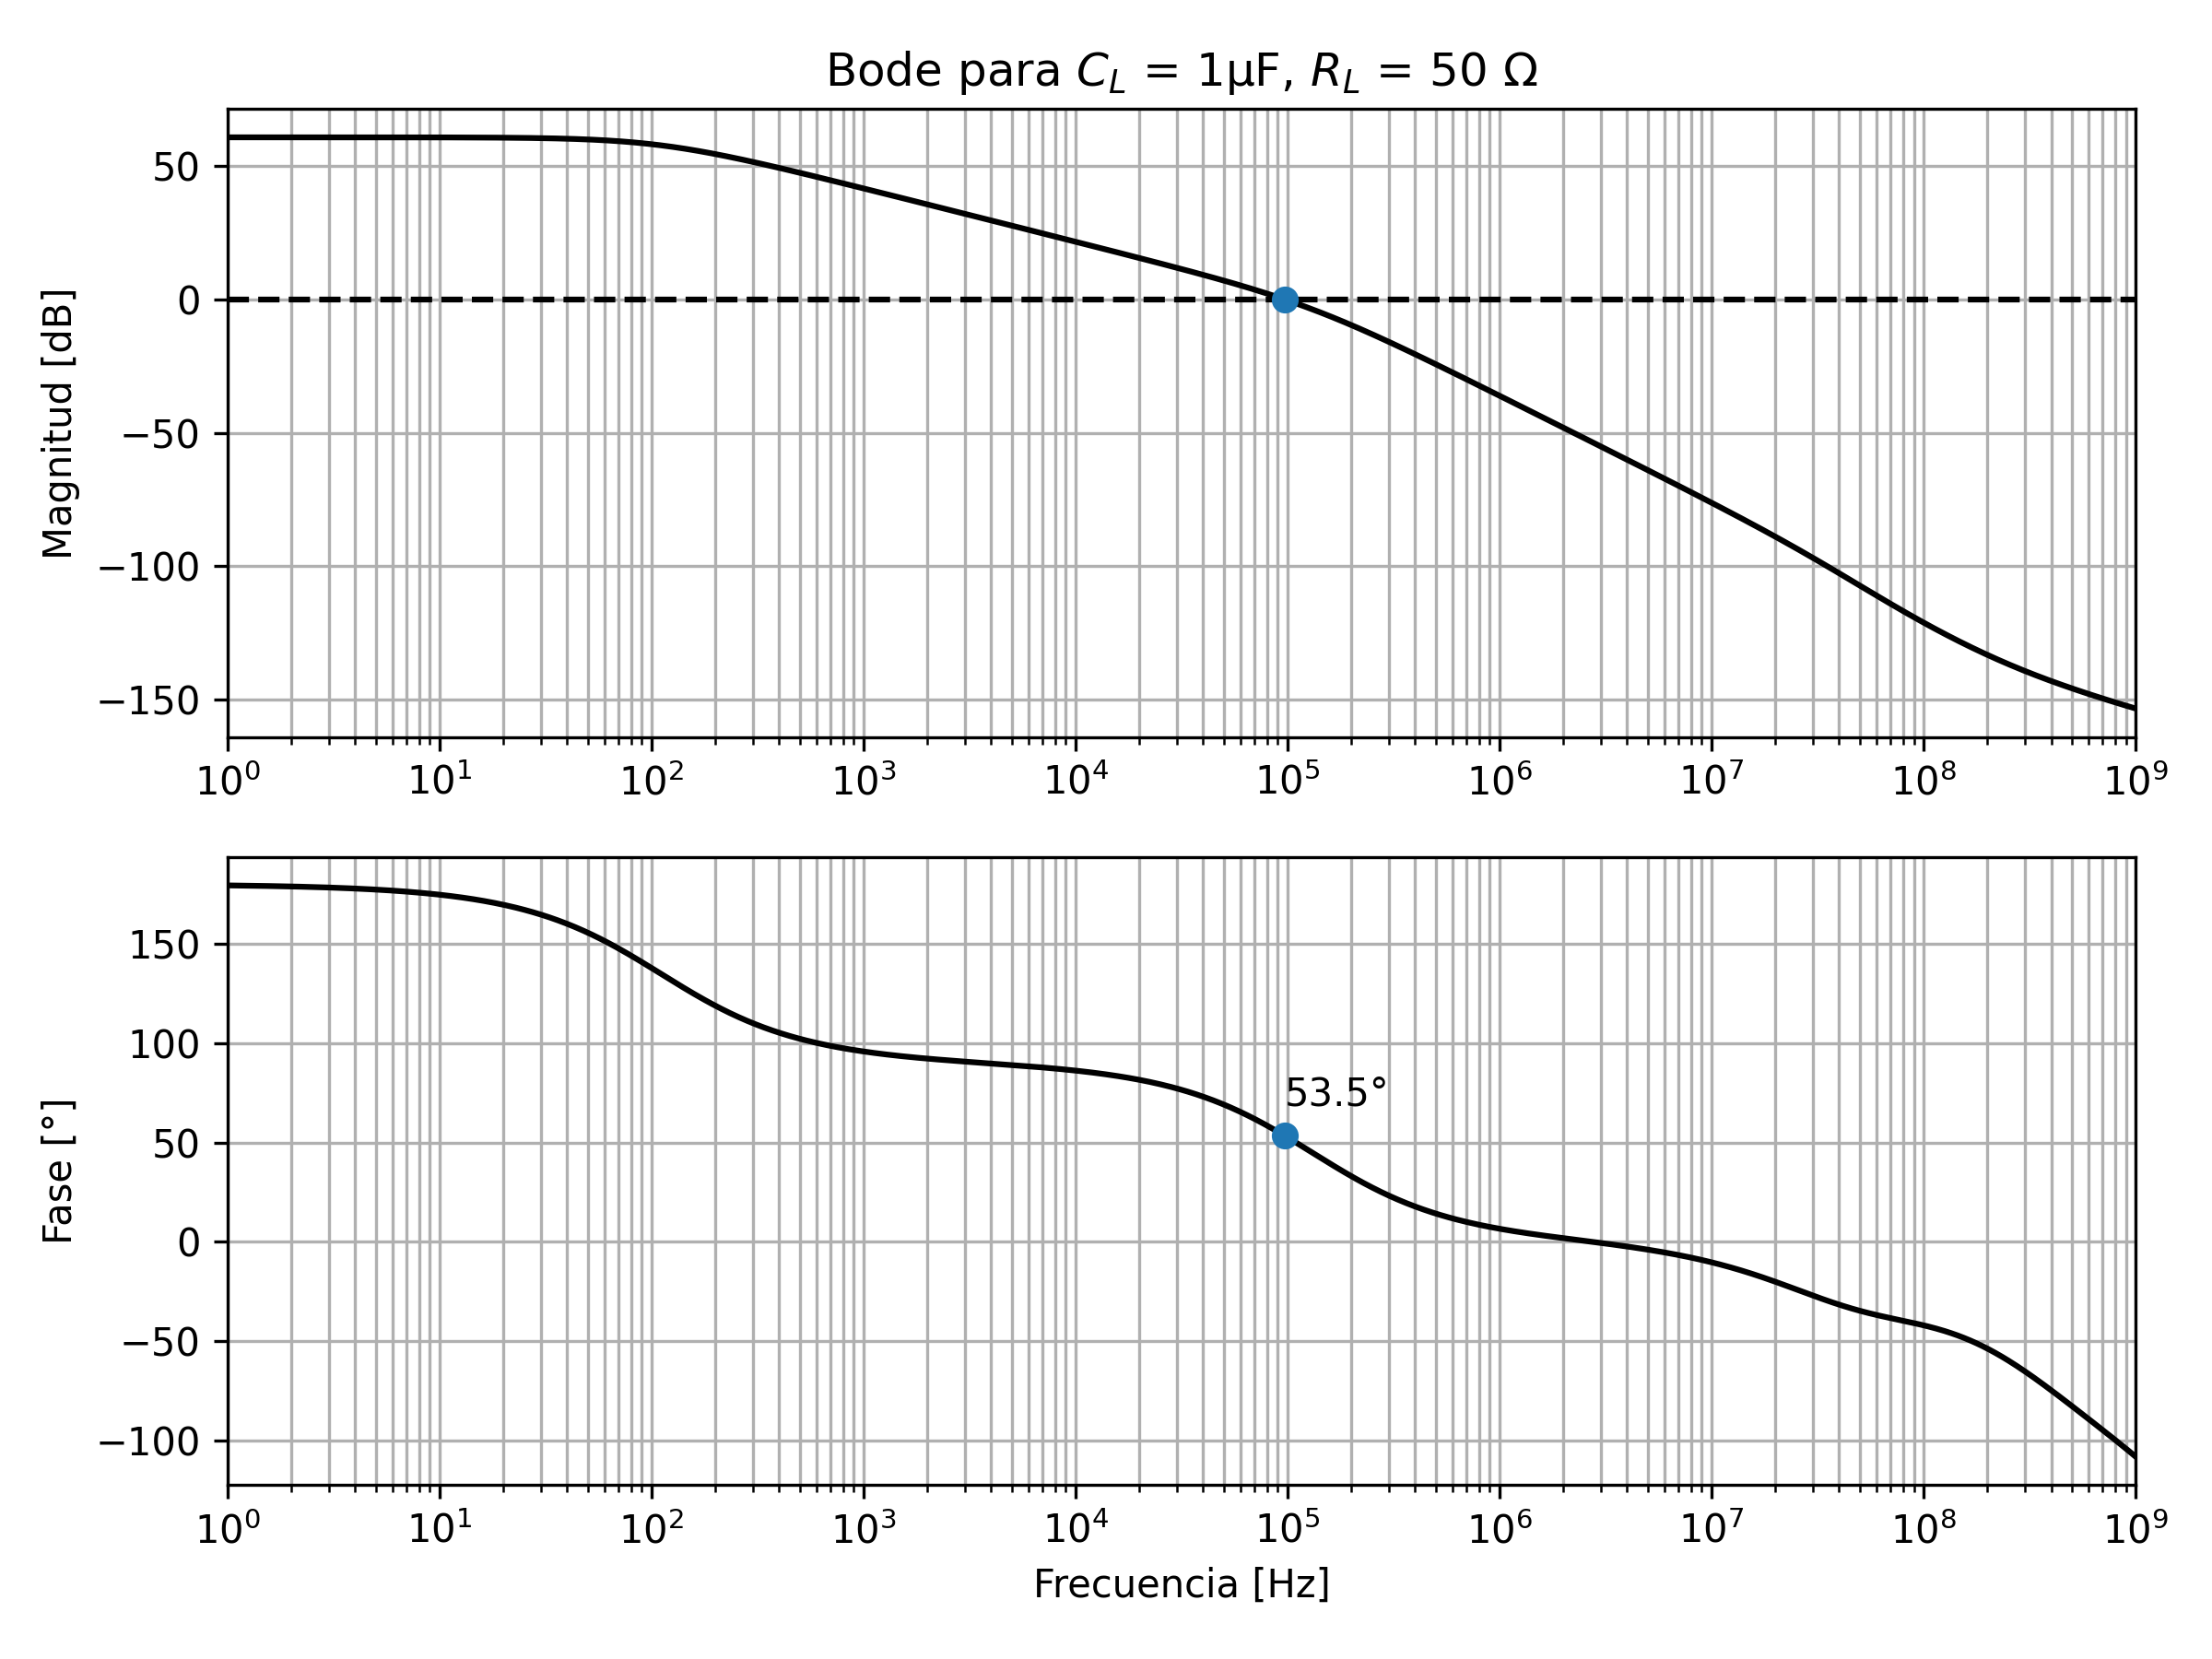
\includegraphics[width=0.9\linewidth]{img/Lazo de tensión/LT compensado.png}
    \caption{Diagrama de Bode del lazo de tensión compensado}
    \label{fig:LT compensado}
\end{figure}

Para apreciar el efecto de la compensación, se simularon las respuestas al escalón del lazo sin compensar y el compensado.

\begin{figure}[H]
    \centering
    
    \begin{subfigure}{0.9\textwidth}
        \centering
        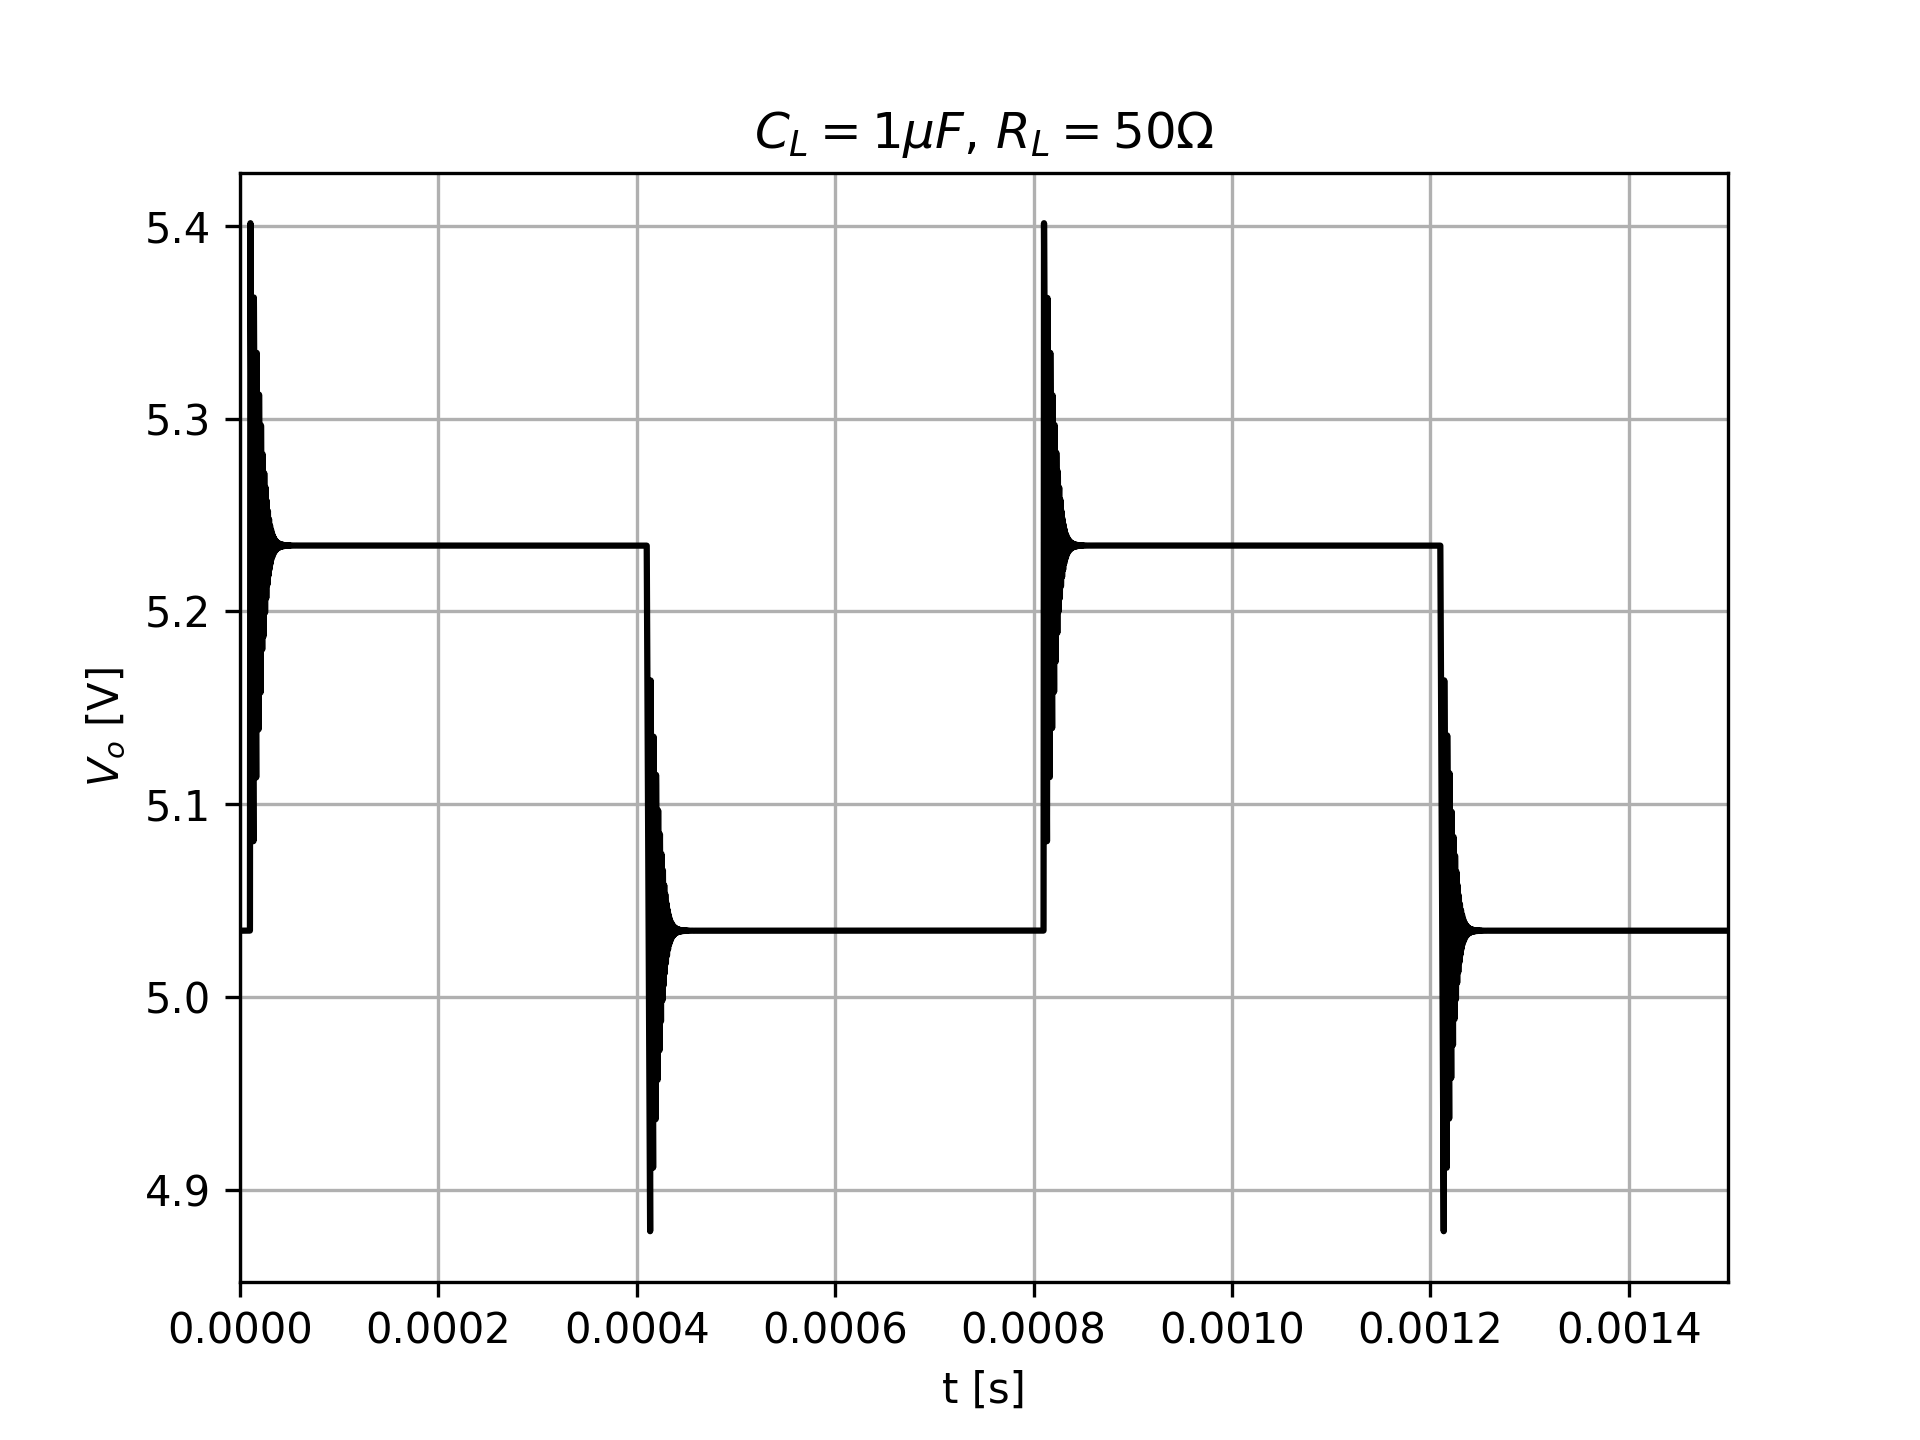
\includegraphics[width=\textwidth]{img/Lazo de tensión/Rta al escalon(sin compensar).png}
        \caption{Respuesta al escalón sin compensar}
        \label{Rta al escalón sin compensar}
    \end{subfigure}
    
    \vspace{0.3cm}
    
    \begin{subfigure}{0.9\textwidth}
        \centering
        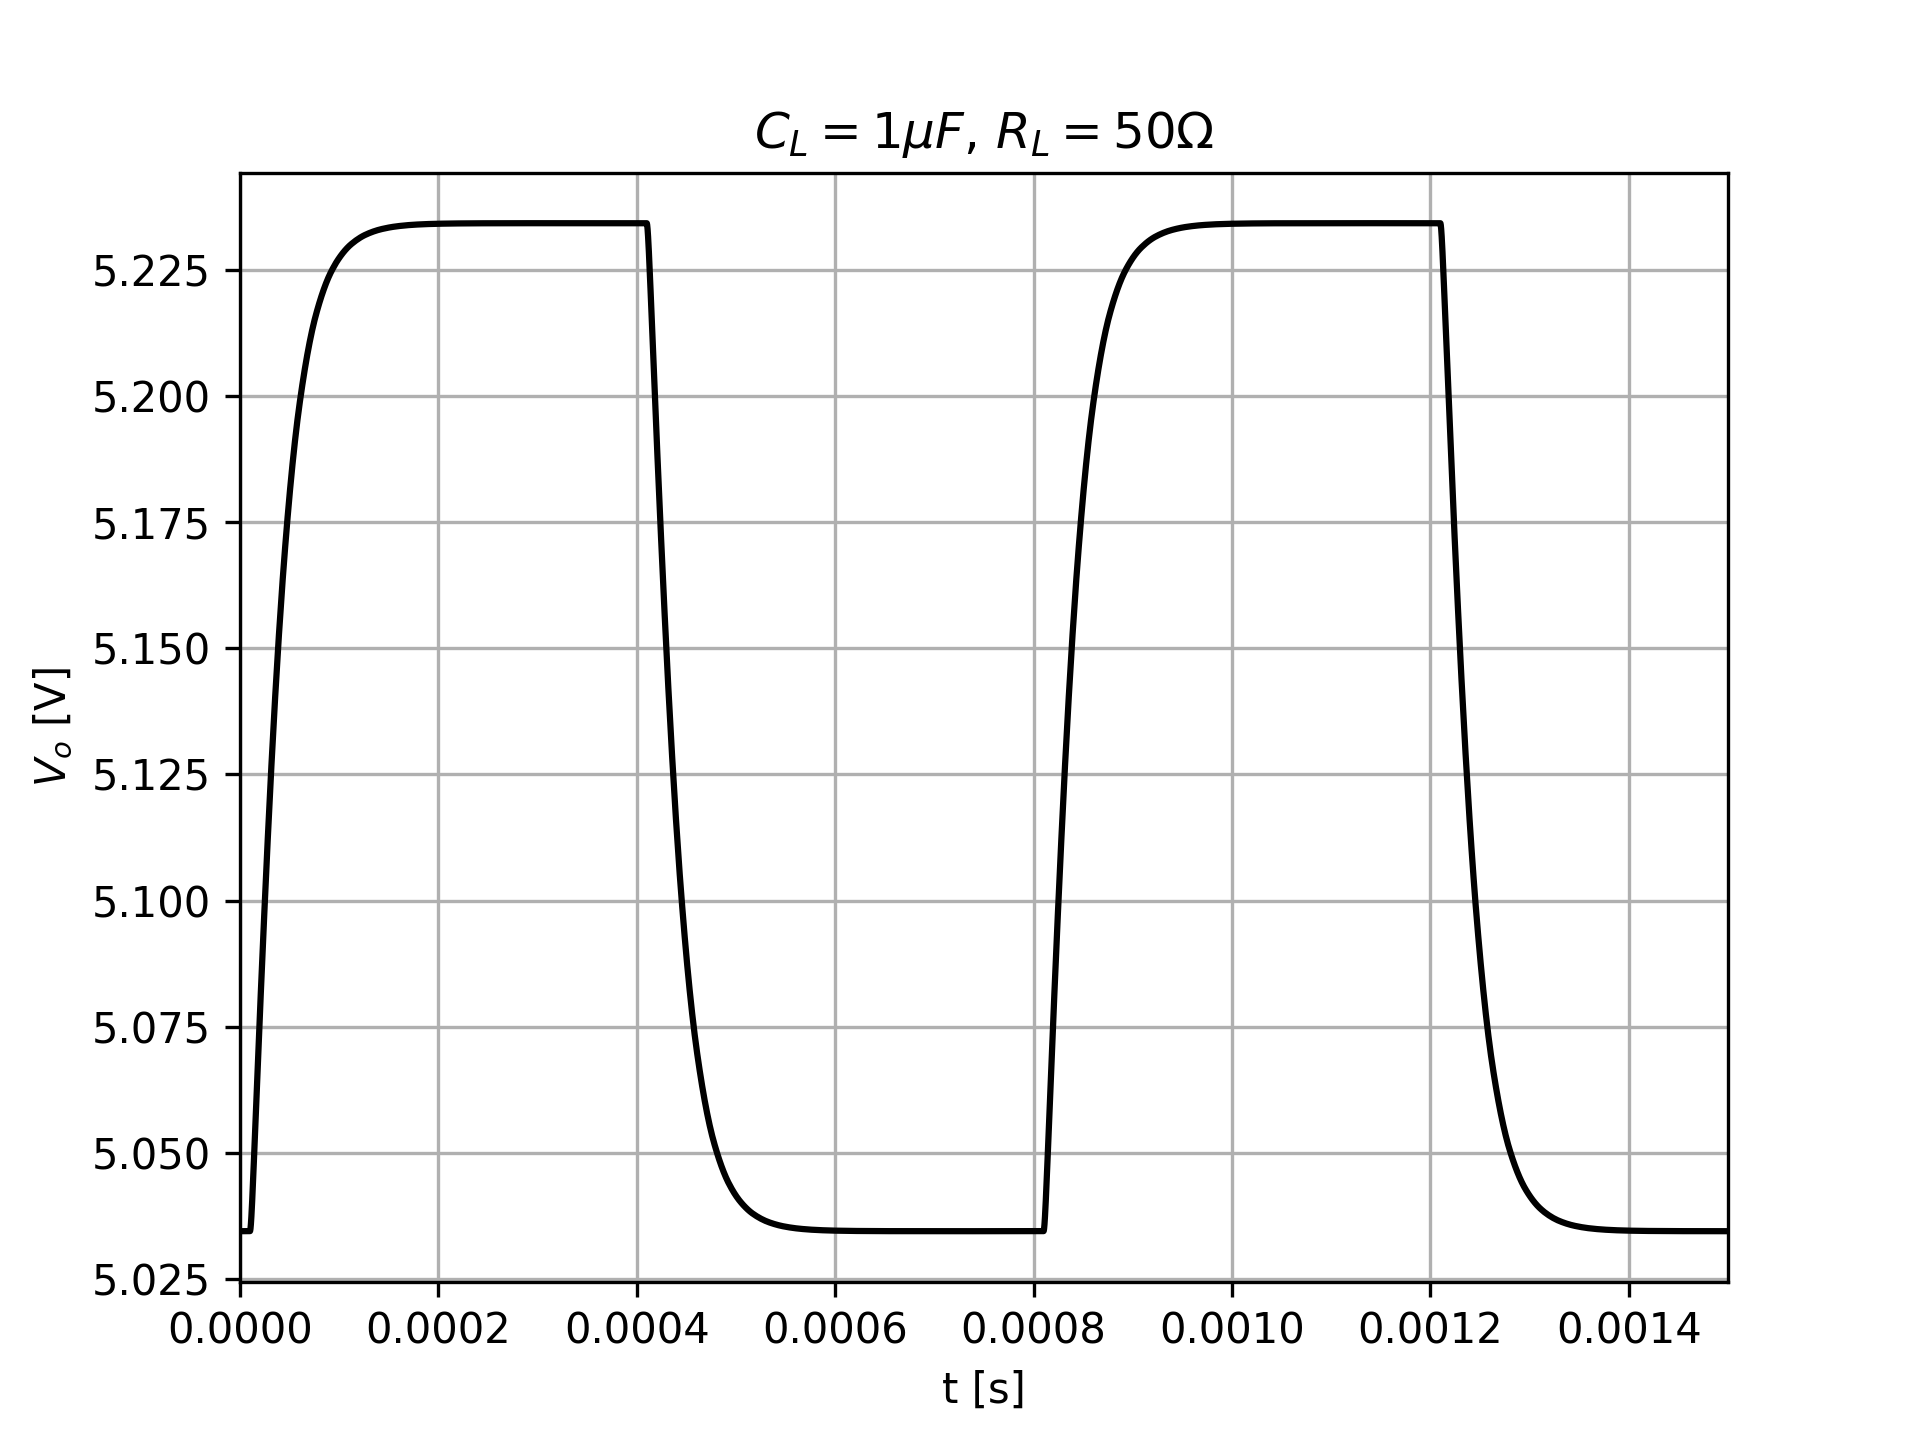
\includegraphics[width=\textwidth]{img/Lazo de tensión/Rta al escalon(compensada).png}
        \caption{Respuesta al escalón compensada}
        \label{Rta al escalon compensada}
    \end{subfigure}
    
    \caption{Respuestas al escalón}
\end{figure}



\subsection{Lazo de corriente}

De forma análoga, se procede a analizar la estabilidad del lazo de corriente. Para ello, se utilizó el circuito de la \autoref{fig:circuito LC}.

\begin{figure}[H]
    \centering
    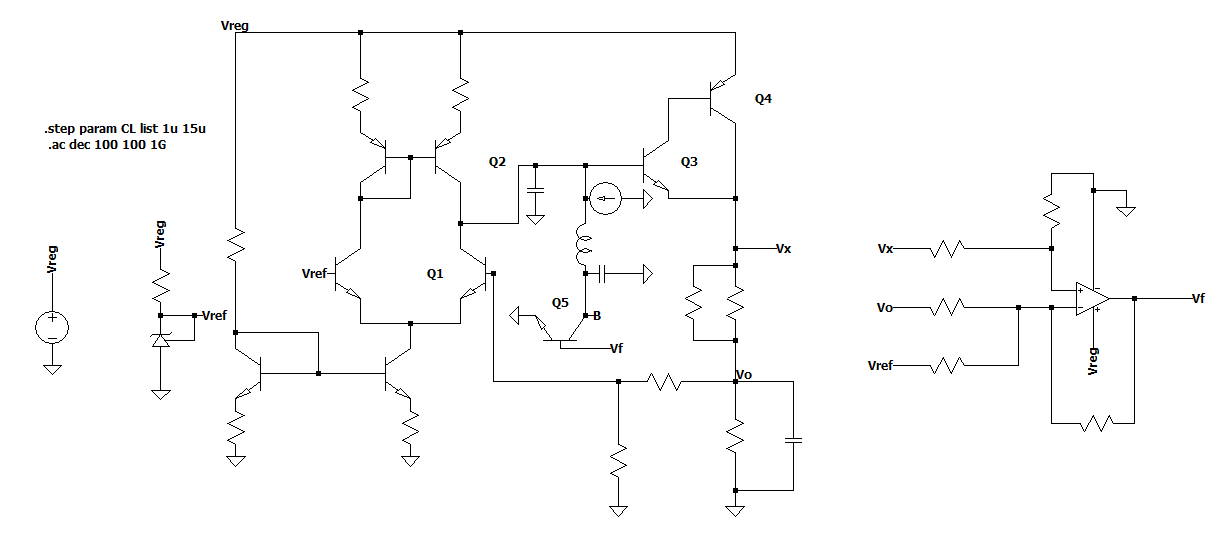
\includegraphics[width=0.9\linewidth]{img/Lazo de corriente/Circuito LC.png}
    \caption{Circutio utilizado para obtener el Bode del lazo de corriente}
    \label{fig:circuito LC}
\end{figure}

Nuevamente, el objetivo es hallar el bode de $L = a \cdot f$. Cabe aclarar que en el lazo de corriente el bloque $a$ son los transistores en configuración cuasi-darlington, mientras que el bloque $f$ está compuesto por la resistencia de sensado, el OpAmp y el transistor de drenaje. Por lo tanto, se abre el circuito entre la base de Q3 y el colector de Q5, se inyecta una corriente alterna y se toma la salida como la corriente del colector de Q5, indicado en la \autoref{fig:circuito LC} como nodo B. De esta forma, se obtuvo el bode de la \autoref{fig:LC sin compensar}. Nuevamente, se compensará el pero caso, que se produce para $C_L = \SI{1}{\micro \farad}$

\begin{figure}[H]
    \centering
    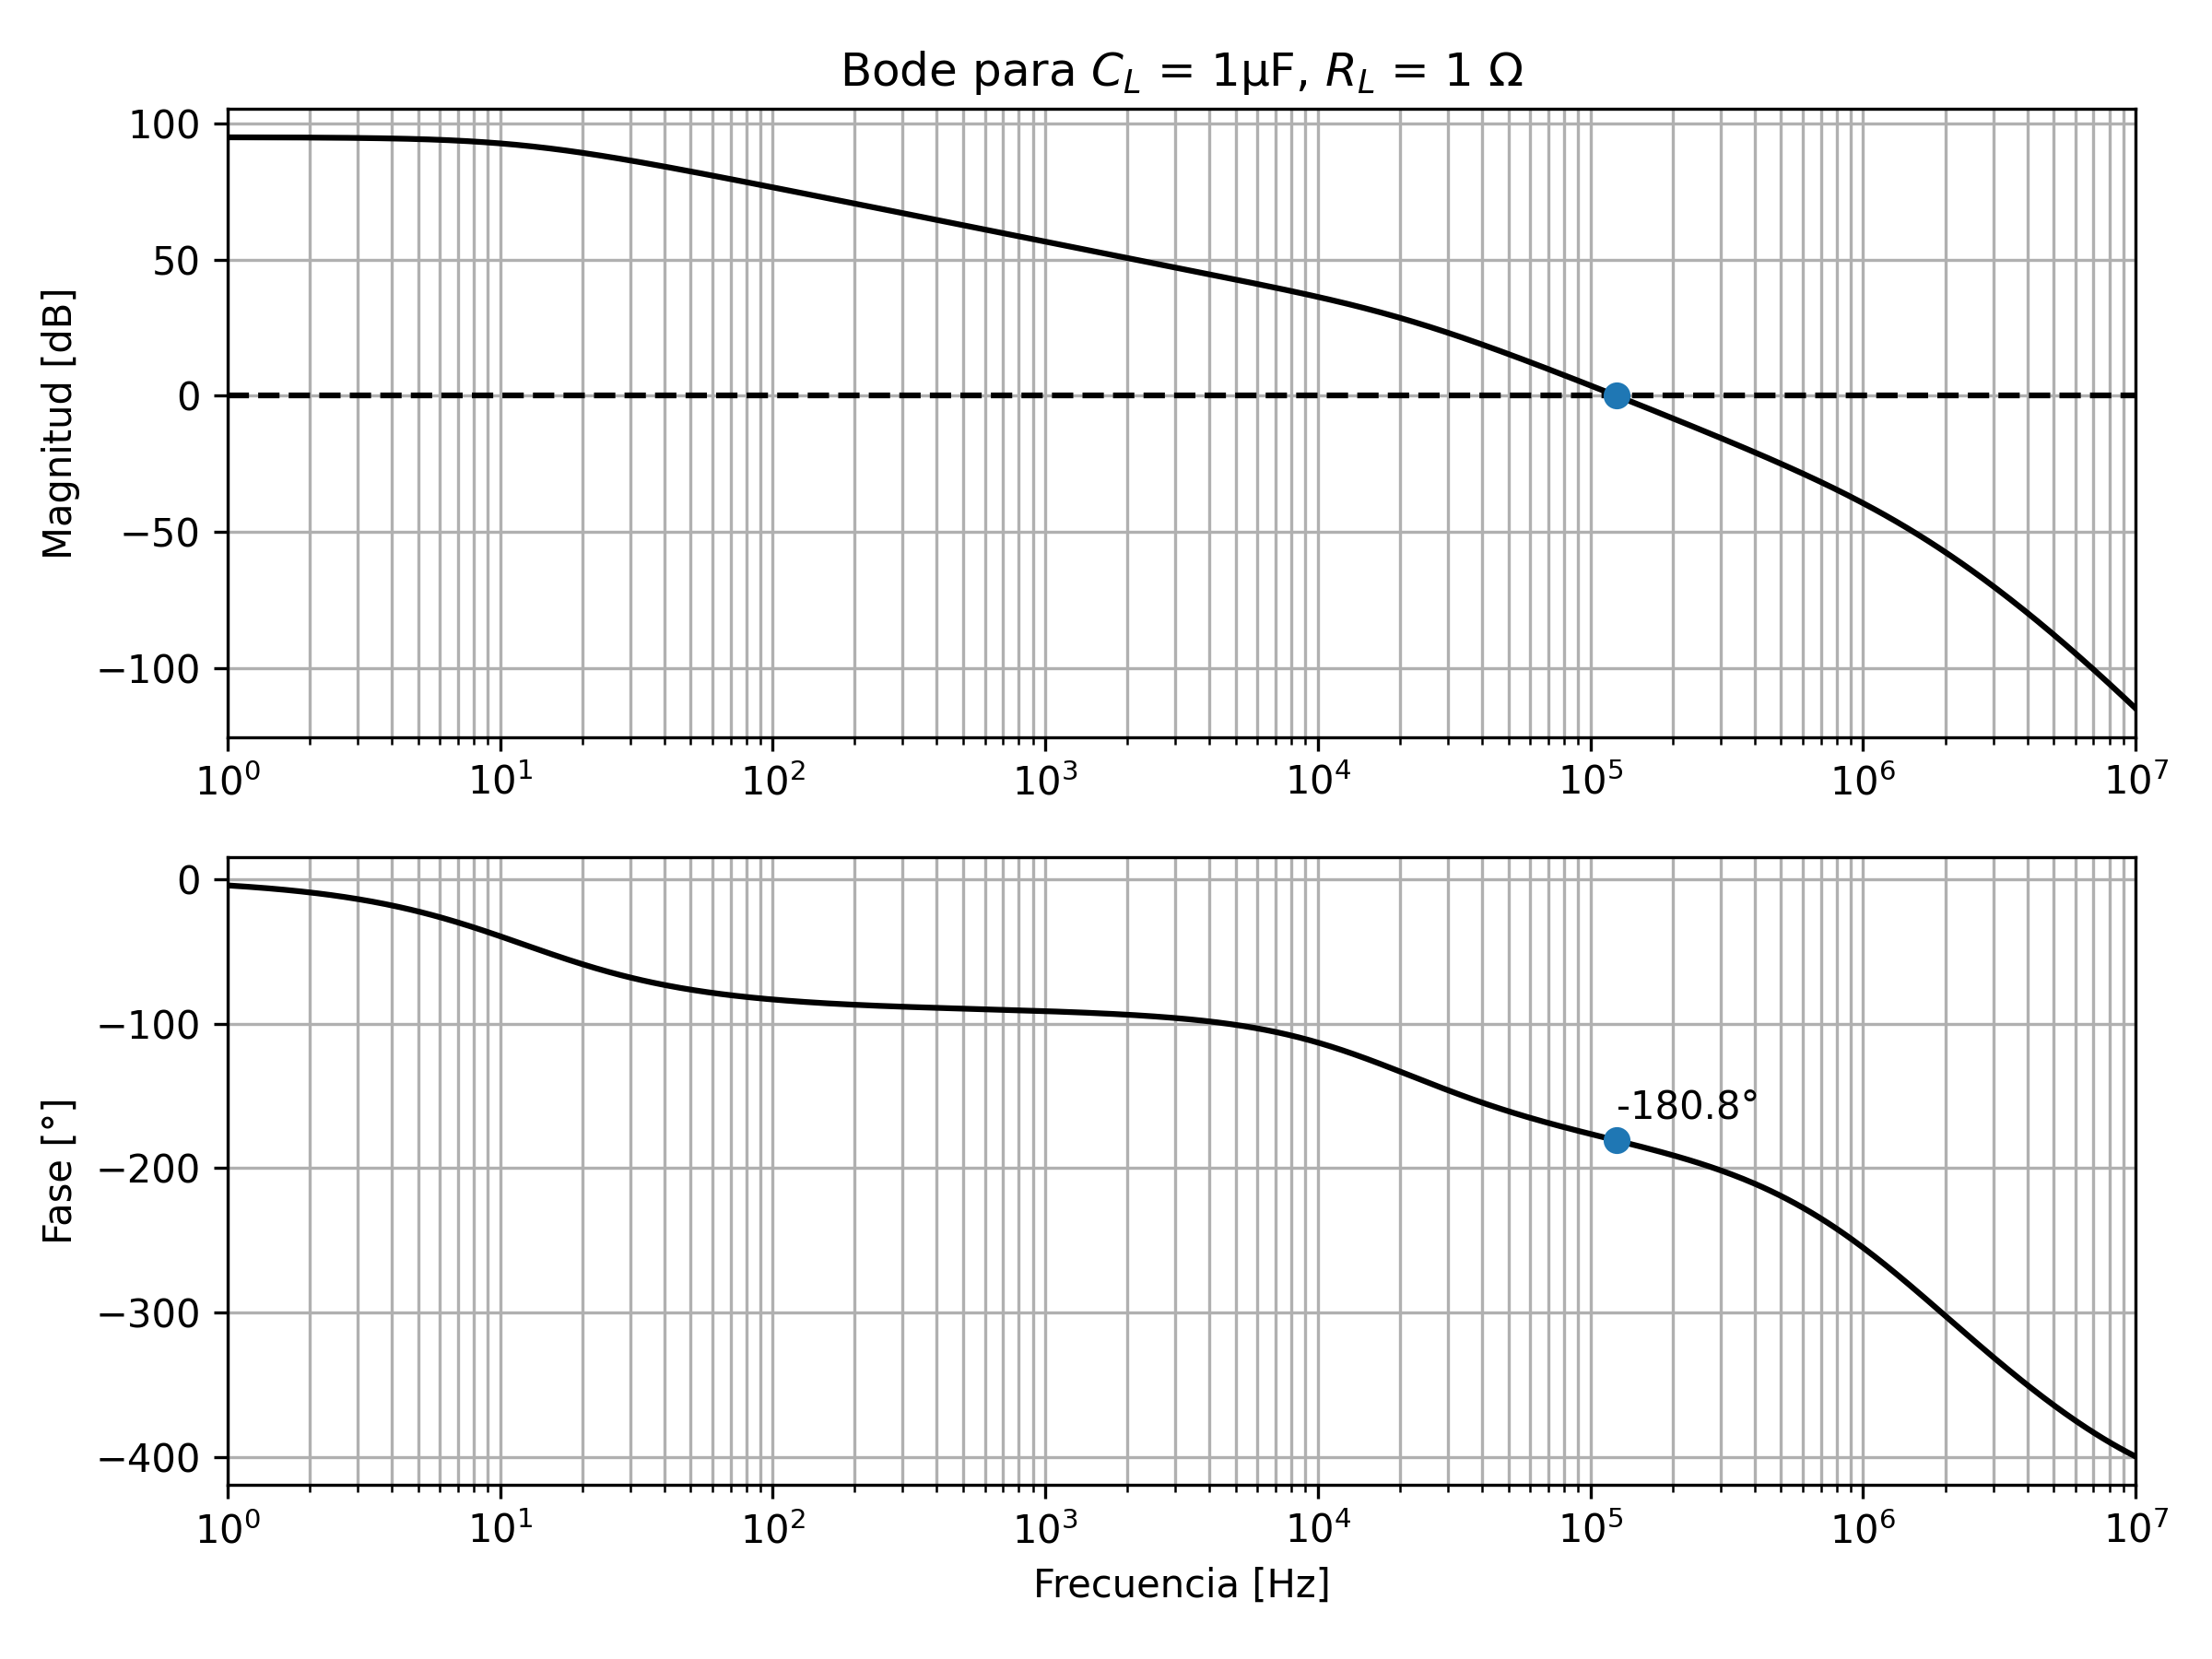
\includegraphics[width=0.9\linewidth]{img/Lazo de corriente/LC sin compensar.png}
    \caption{Lazo de corriente sin compensar}
    \label{fig:LC sin compensar}
\end{figure}

De este gráfico se concluye que es necesario añadir fase en las frecuencias del orden de los \SI{100}{\kilo \hertz}, por lo que debe añadirse un cero una década antes. Se añadirá entonces una resistencia en serie con el capacitor de \SI{330}{\nano \farad} ya agregado. De esta forma, se obtendría un cero en $z = \frac{1}{2\pi R C}$. De esta cuenta se despeja la resistencia para obtener un rango aproximado para la misma.

\begin{equation}
    R = \frac{1}{2\pi C z} = \frac{1}{2\pi \cdot \SI{330}{\nano \farad} \cdot \SI{10}{\kilo \hertz}} \approx  50 \Omega
\end{equation}

Por lo tanto, se necesita una resistencia del orden de las decenas de Ohm. Probando distintos valores comerciales, se obtiene que para $R = $ \SI{22}{\ohm} el lazo se estabiliza satisfactoriamente. En las Figuras \ref{fig: LC compensado CL=1uF}  y \ref{fig: LC compensado CL = 15uF} se muestran los diagrama de bode del lazo de corriente compensado para ambos casos de la capacidad de carga.

\begin{figure}[H]
    \centering
    
    \begin{subfigure}{0.9\textwidth}
        \centering
        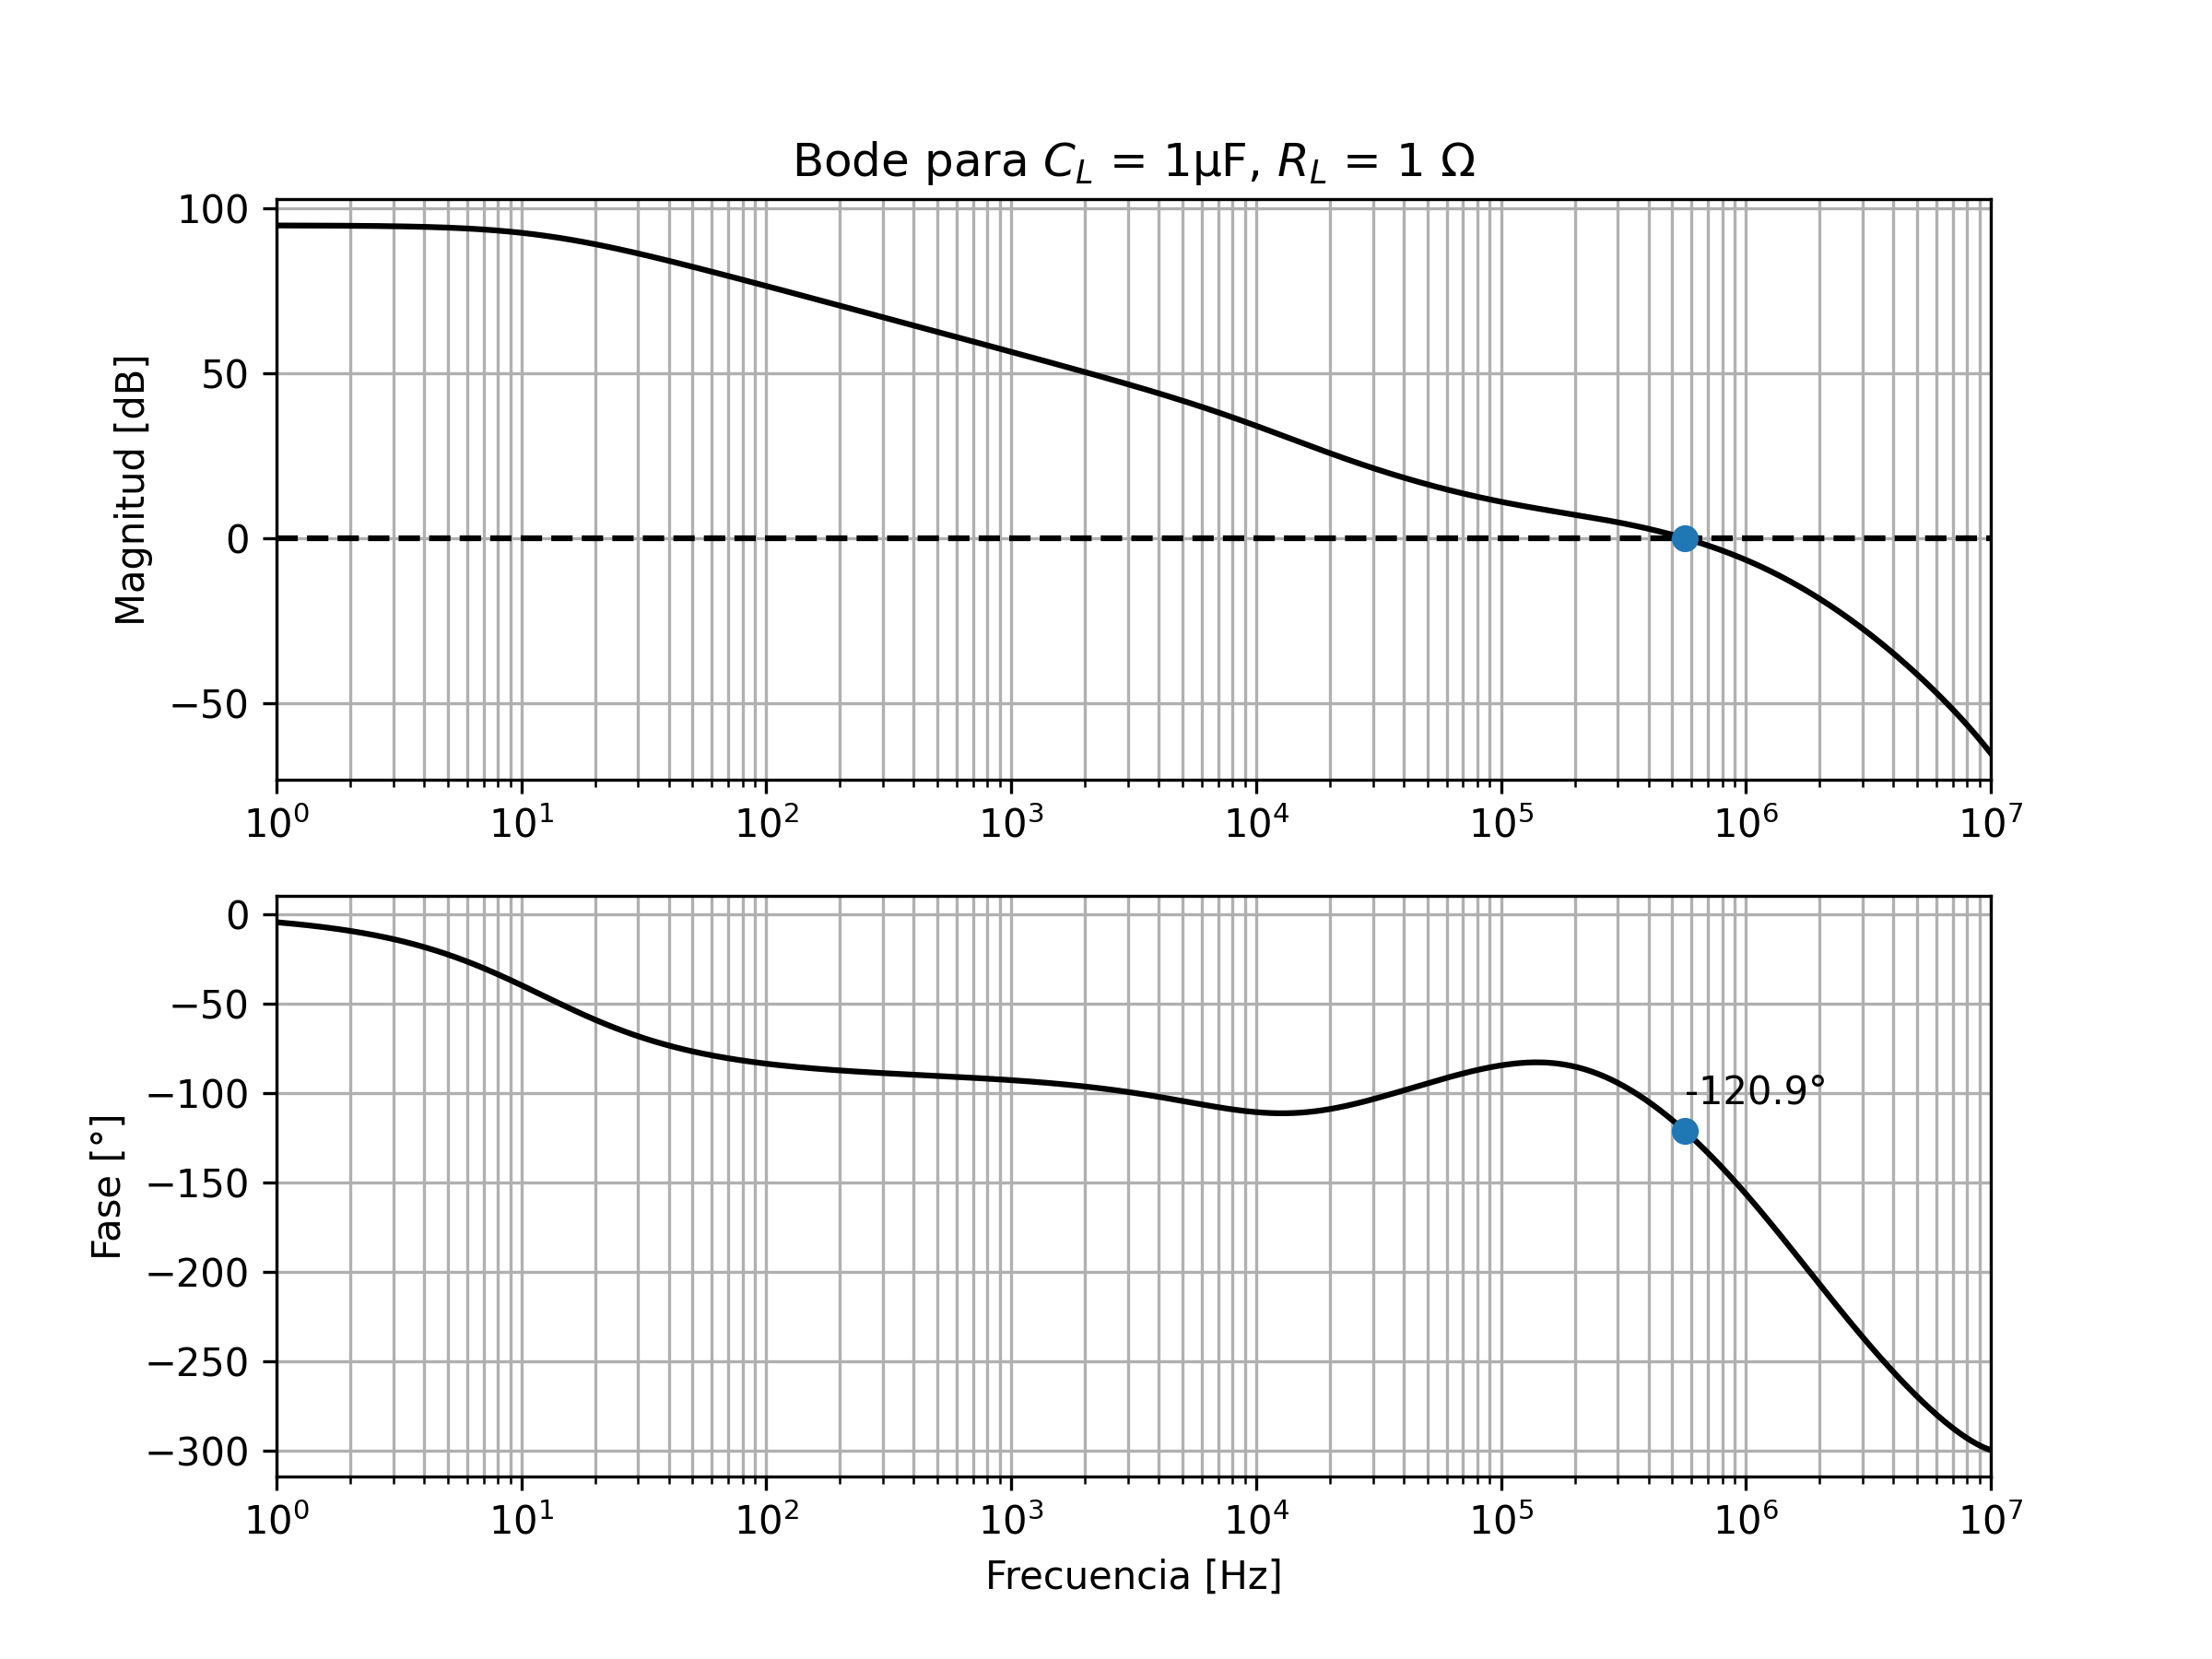
\includegraphics[width=\textwidth]{img/Lazo de corriente/LC compensado 1uF.png}
        \caption{Lazo de corriente compensado para $C_L = 1 \mu F$}
        \label{fig: LC compensado CL=1uF}
    \end{subfigure}
    
    \vspace{0.3cm}
    
    \begin{subfigure}{0.9\textwidth}
        \centering
        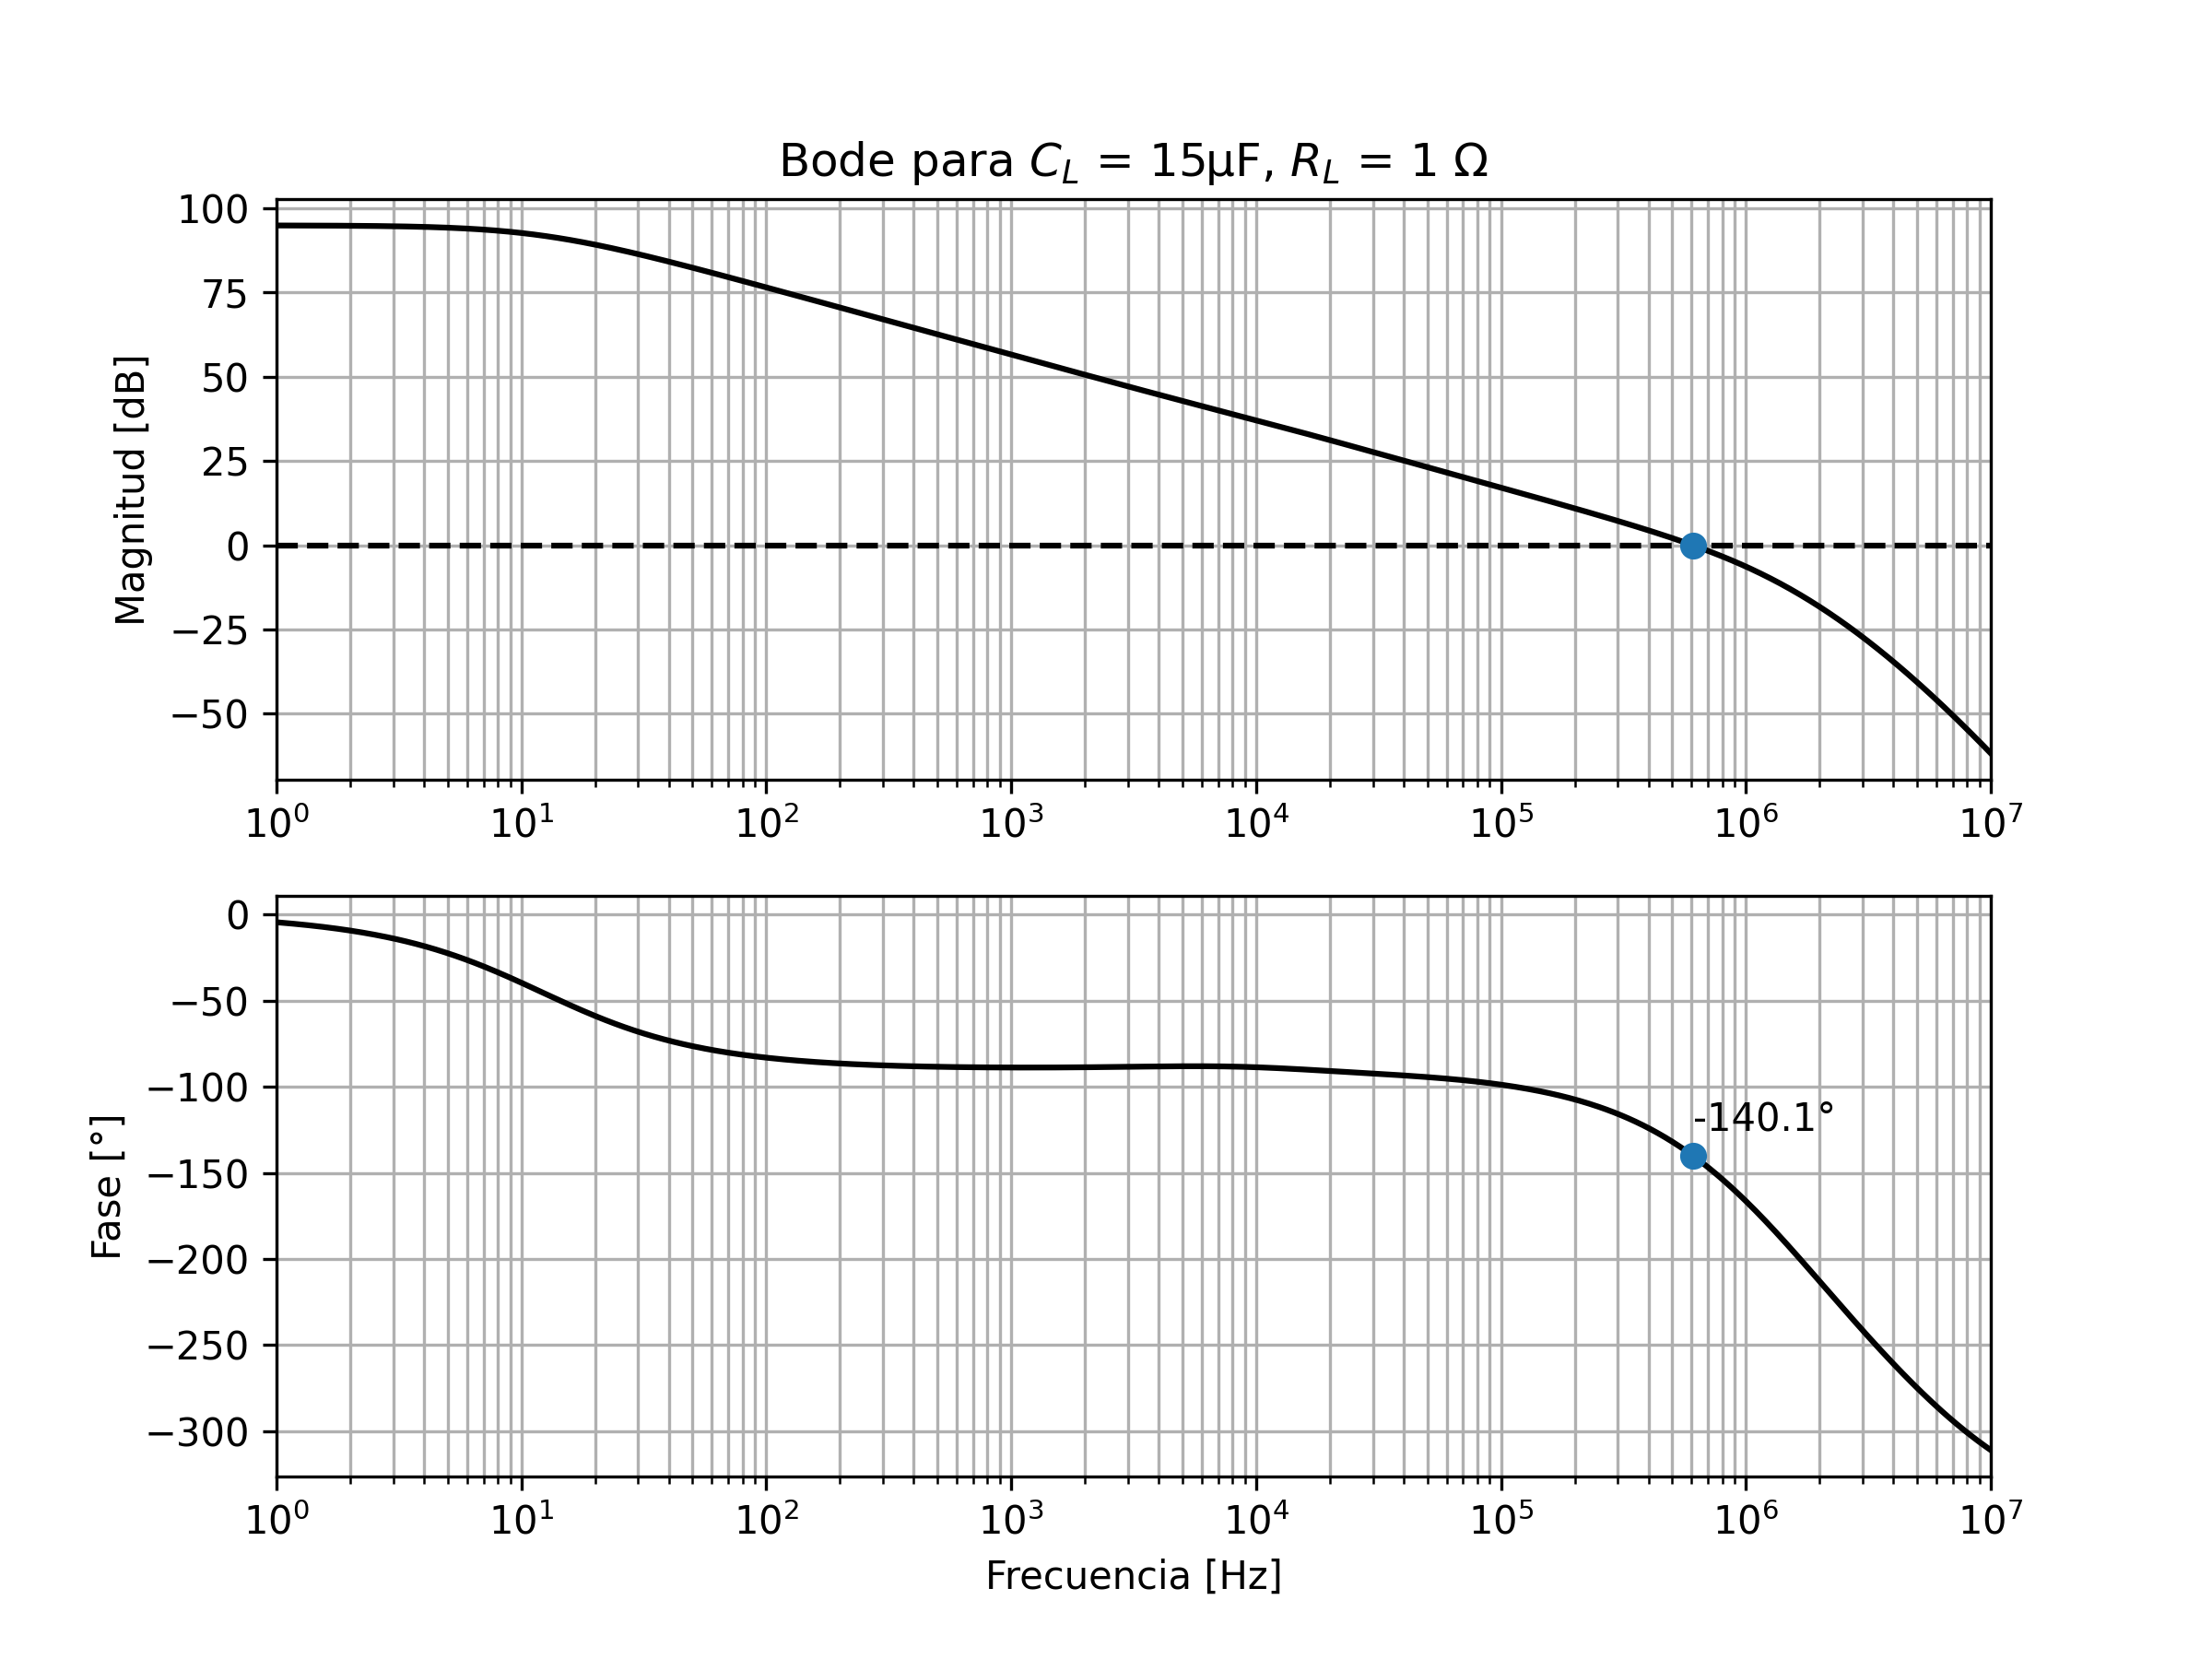
\includegraphics[width=\textwidth]{img/Lazo de corriente/LC compensado 15uF.png}
        \caption{Lazo de corriente compensado para $C_L = 15\mu F$}
        \label{fig: LC compensado CL = 15uF}
    \end{subfigure}
    
    \caption{Lazos de corriente compensados}
\end{figure}

Puede notarse que ahora, el pero caso se da para $C_L =  \SI{15}{\micro \farad} $. Finalmente, se simuló la respuesta al escalón para el circuito con y sin compensación. El circuito usado puede verse en la figura \ref{fig:circuito rta al escalon LC}

\begin{figure}[H]
    \centering
    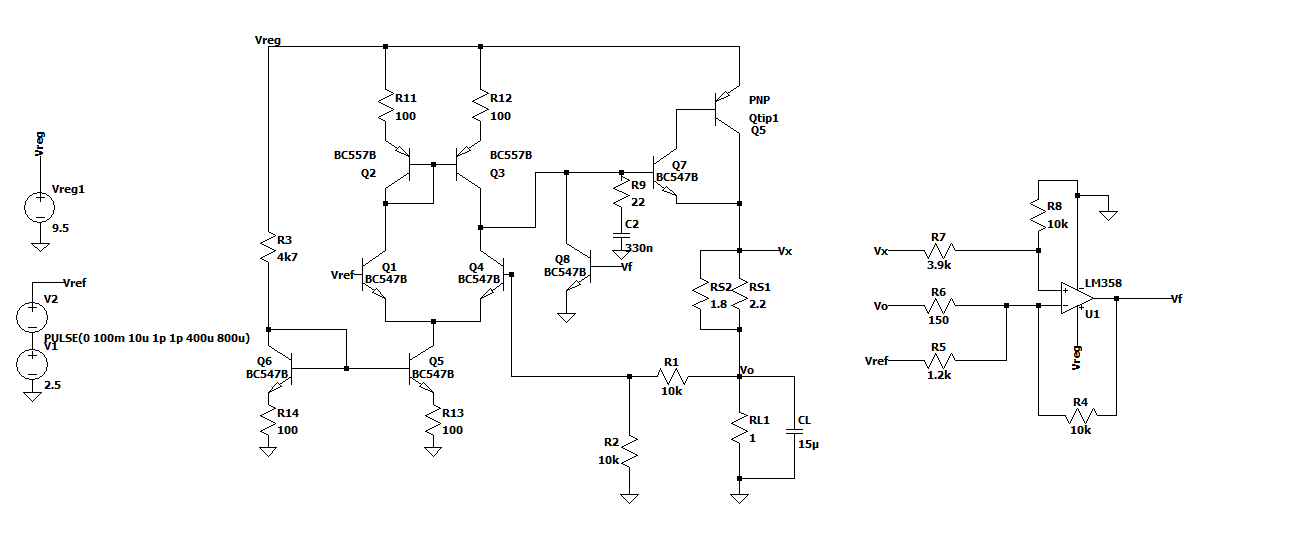
\includegraphics[width=0.9\linewidth]{img/Lazo de corriente/Circuito LC rta al escalon.png}
    \caption{Circuito utilizado para medir la respuesta al escalón}
    \label{fig:circuito rta al escalon LC}
\end{figure}

\begin{figure}[h]
    \centering

    \begin{subfigure}{0.45\textwidth}
        \centering
        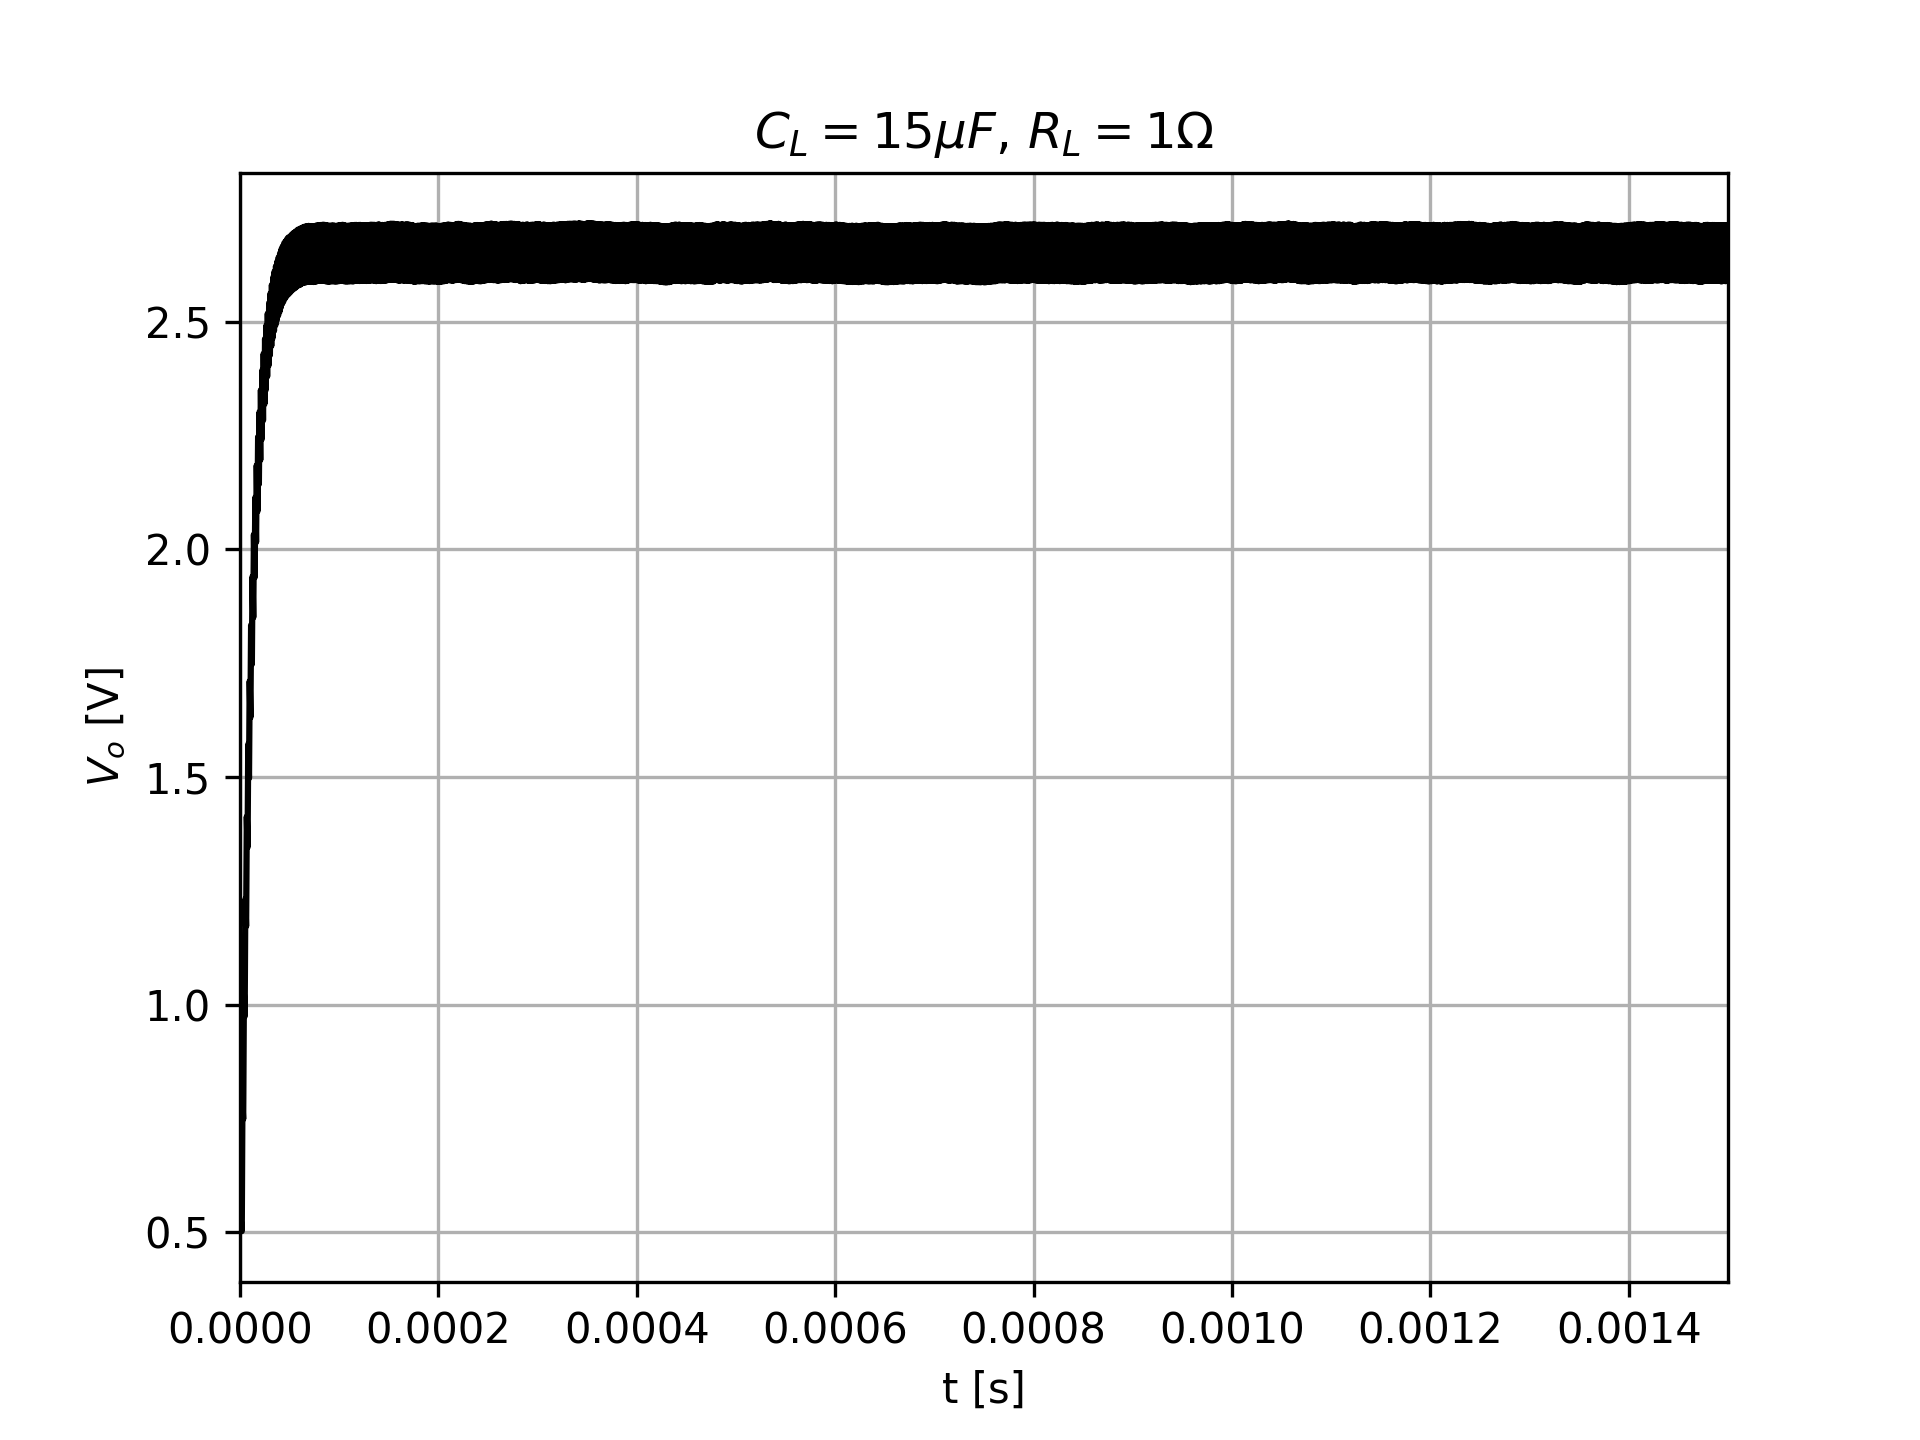
\includegraphics[width=\linewidth]{img/Lazo de corriente/Rta al escalon LC (sin compensar).png}
        \caption{Respuesta al escalón sin compensar}
    \end{subfigure}
    \hfill
    \begin{subfigure}{0.45\textwidth}
        \centering
        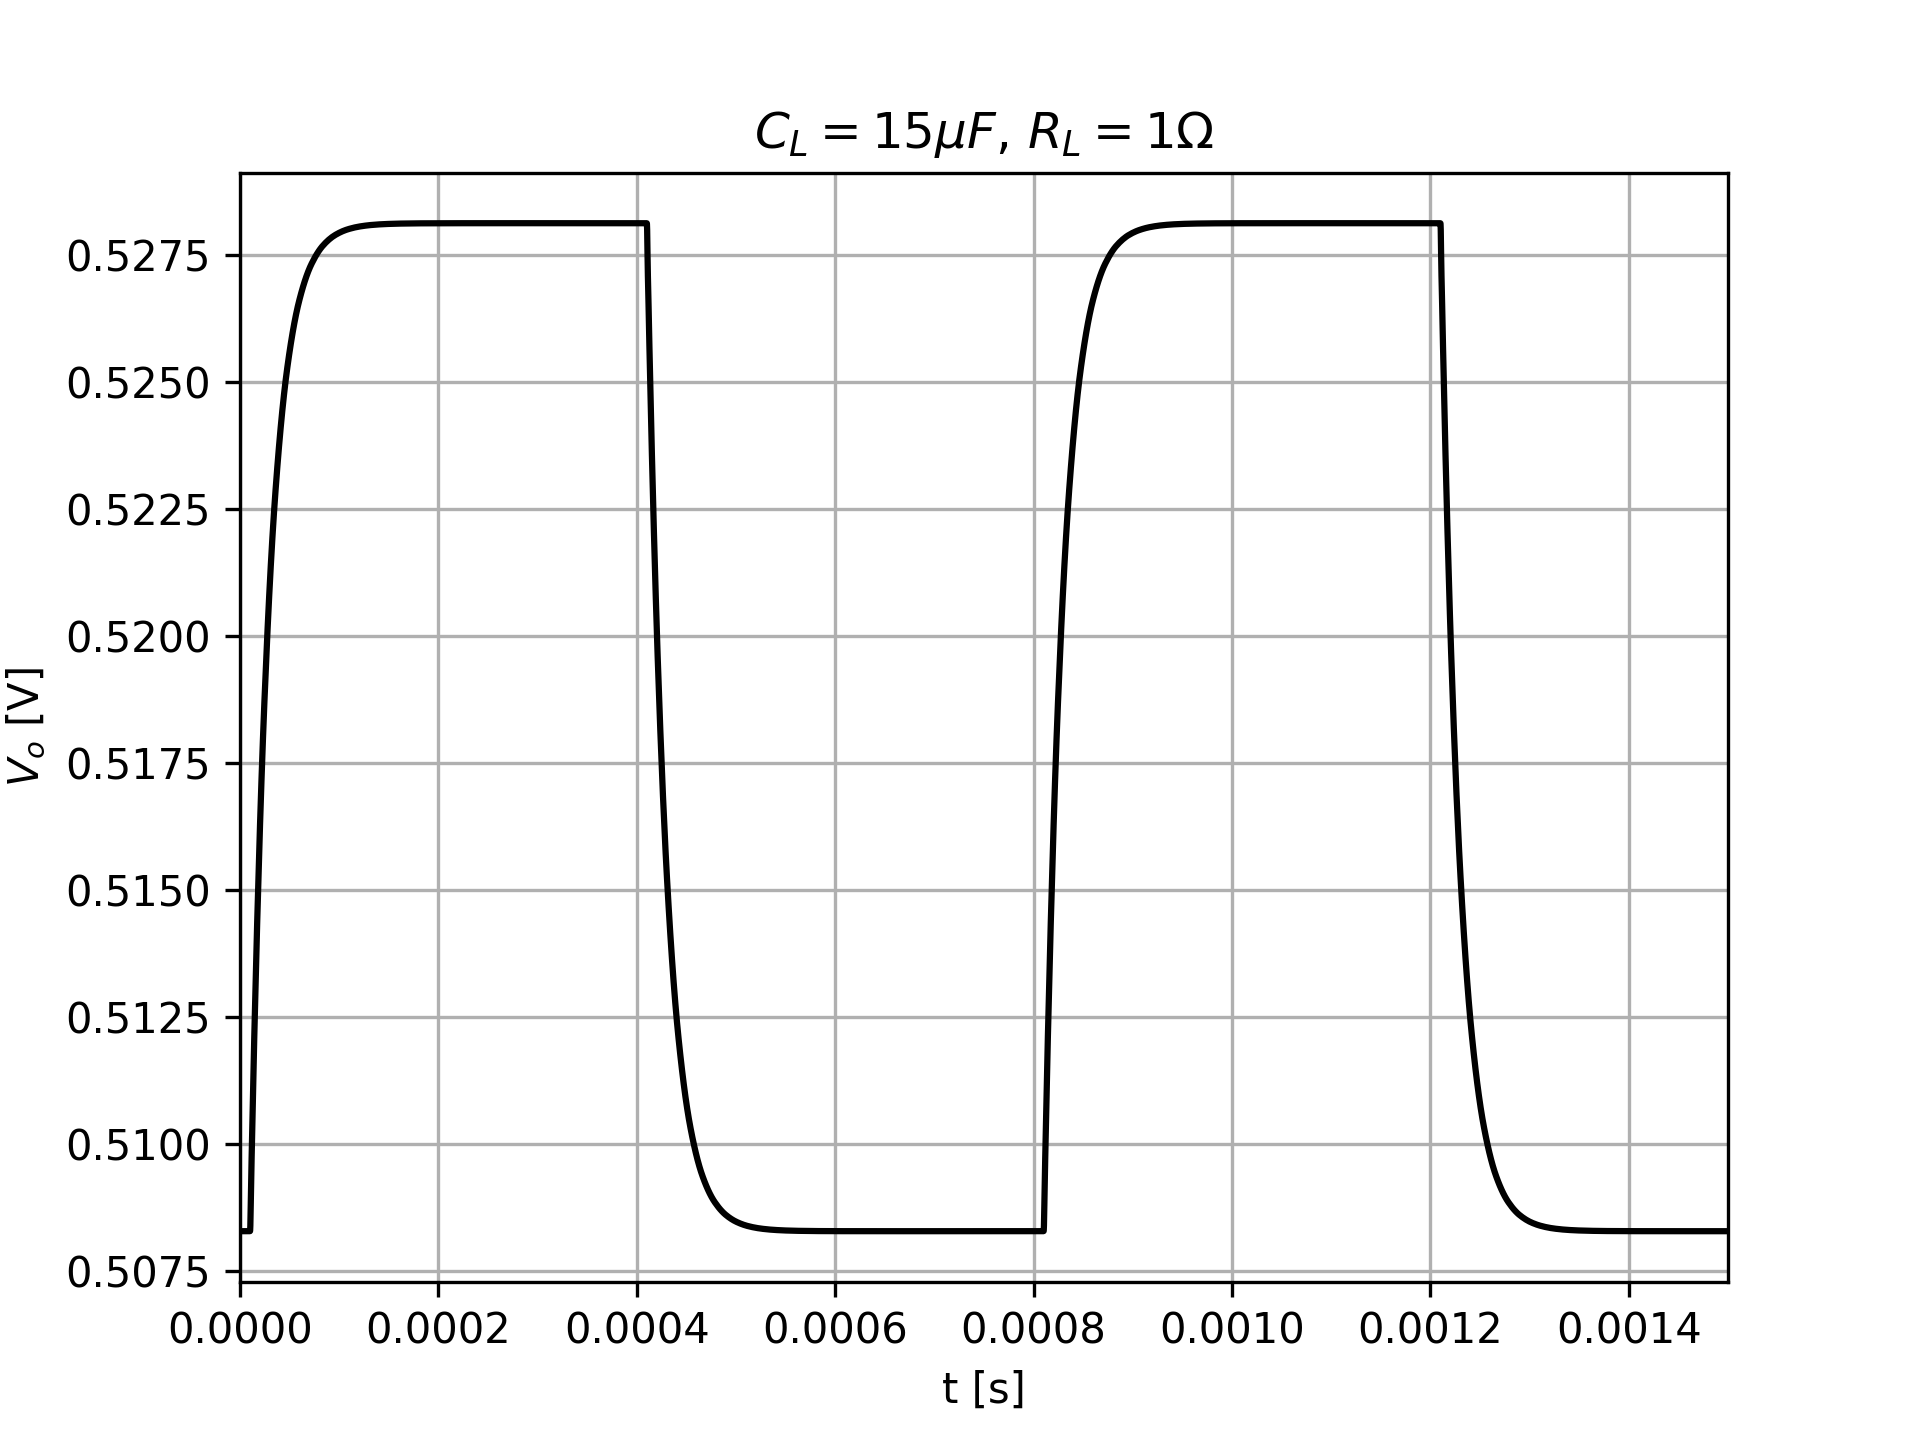
\includegraphics[width=\linewidth]{img/Lazo de corriente/Rta al escalon LC(compensada).png}
        \caption{Respuesta al escalón compensada}
    \end{subfigure}

    \caption{Respuestas al escalón}
\end{figure}

\section{Análisis térmico y elección del disipador}

Según la hoja de datos del TIP32, la temperatura de juntura máxima $\left(T_j^\text{max}\right)$ es de 150 °C, la resistencia térmica juntura-a-ambiente máxima $\left(\theta_{ja}^\text{max}\right)$ es 62,5 °C/W y la resistencia térmica juntura-a-carcasa máxima $\left(\theta_{jc}^\text{max}\right)$ es 3,125 °C/W. Esto corresponde a una potencia disipada máxima $P_d^\text{max} = 2\,\text{W}\quad@\quad T_{a} = 25\,\text{°C}$ y $P_d^\text{max} = 40\,\text{W}\quad@\quad T_{c} = 25\,\text{°C}$.

La tensión del transistor de paso es la siguiente.

\begin{align*}
    V &= V_\text{REG} - I R_S - V_O \\
      & = 4,5\,\text{V} - 990\,\text{m}\Omega\,I
\end{align*}

De esta forma, la potencia que consume es 

\[
P_c = V\cdot I = 4,5\,\text{V}\, I - 990\,\text{m}\Omega\,I^2,
\]

por lo que para calcular la potencia consumida máxima basta con encontrar el máximo de esa parábola, teniendo en cuenta que el circuito está limitado a una corriente de 1,5 A y que se adopta un único sentido de flujo positivo.

\[
P_c^\text{max} = \max_{0 \le I \le 1,5\,\text{A}} P_c(I) = 4,5225 \, \text{W} \quad @ \quad I = 1,5 \, \text{A}
\]

En la Figura \ref{fig:disipador} se observa el modelo aplicado al cálculo del disipador mediante la Ley de Ohm Térmica.

\begin{figure}[H]
    \centering
    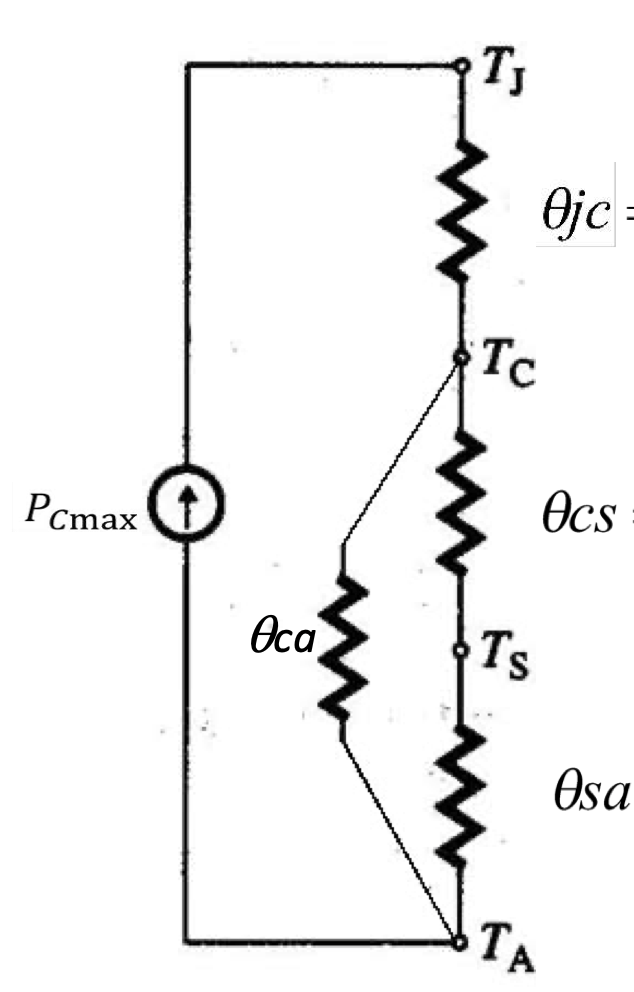
\includegraphics[scale = 0.4]{img/ley_ohm_termica.png}
    \caption{Modelo de la Ley de Ohm Térmica.}
    \label{fig:disipador}
\end{figure}

Nótese que generalmente $\theta_{ca}$ es mucho mayor que $\theta_{cs} + \theta_{sa}$, por lo que se desprecia.  

Suponiendo un caso extremo de temperatura ambiente $T_a = 38,5$ °C, se obtiene

\[
\theta_{ja} = \frac{T_j - T_a}{P_c^\text{max}} \approx 24,65 \, \text{°C/W}\,.
\]

La resistencia térmica disipador-a-ambiente $\left(\theta_{sa}\right)$ es la informada por el fabricante, la cual se obtiene como

\[
\theta_{sa} = \theta_{ja} - \theta_{jc} - \theta_{cs}\,.
\]

La resistencia carcasa-a-disipador $\left(\theta_{cs}\right)$ se va a minimizar usando mica con grasa térmica ($\sim$0,5 °C/W), por lo que se obtiene 

\[
\theta_{sa} \approx 21 \, \text{°C/W}\,.
\]

El disipador D-5235FD tiene exactamente esa resistencia térmica, por lo que es el elegido. Además, sus dimensiones son de $(20\times20\times20)$ mm y su espesor es de 1,5 mm.

\section{Diseño del PCB}

Sobre el diseño hecho previamente se desarrolló un PCB en \texttt{KiCAD}. 

\begin{figure}[H]
    \centering

    \begin{subfigure}{0.45\textwidth}
        \centering
        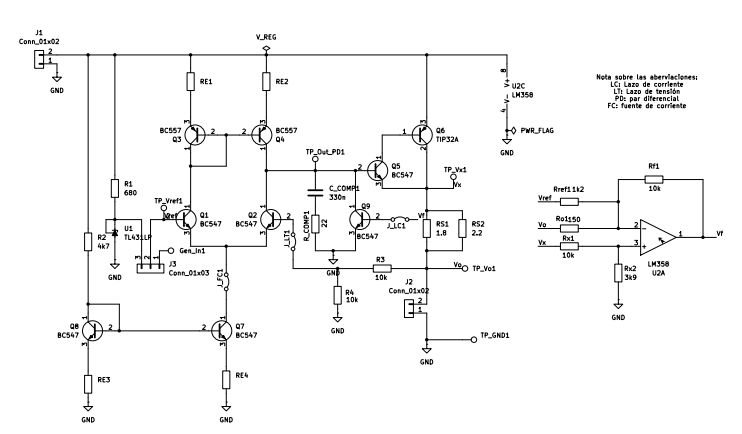
\includegraphics[width=\linewidth]{img/KiCAD/Esquemático.png}
        \caption{Esquemático}
    \end{subfigure}
    \hfill
    \begin{subfigure}{0.45\textwidth}
        \centering
        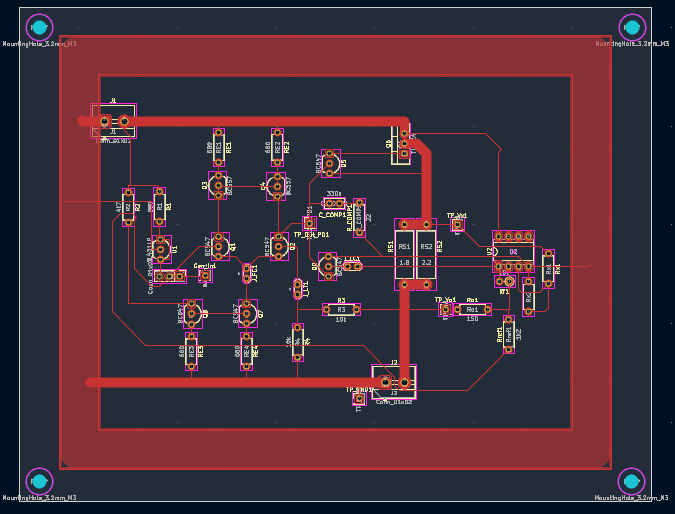
\includegraphics[width=\linewidth]{img/KiCAD/PCB.png}
        \caption{PCB}
    \end{subfigure}

    \caption{PCB diseñado en \texttt{KiCAD}}
\end{figure}

\begin{figure}[H]
    \centering
    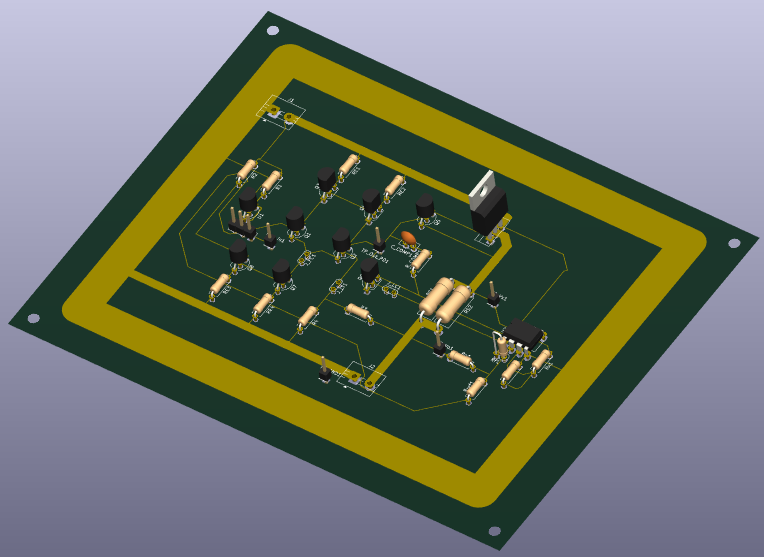
\includegraphics[width=0.9\linewidth]{img/KiCAD/PCB 3D.png}
    \caption{PCB}
\end{figure}

El PCB cuenta con un anillo de tierra que rodea a todos los componentes. El mismo reduce la interferencia electromagnética y permite acceder fácilmente al nodo de tierra desde cualquier componente. Además, cabe destacar que la pista que une al transistor de paso con la carga es de un ancho mayor, ya que por la misma podrías circular hasta \SI{1,5}{\ampere}. Por último, para los resistores que forman la resistencia de sensado se eligieron modelos capaces de disipar toda la potencia necesaria (hasta \SI{2}{\watt}). 

\section{Conclusiones}

En este informe se analizó la estabilidad de los lazos de tensión y corriente desarrollados en la entrega anterior. Ambos resultaron inestables o presentaron márgenes de fase muy pequeños, por lo que fue necesario compensar con una red RC. 

En cuanto al lazo de tensión, el peor de los casos presenta un margen de fase de 53° luego de la compensación.

Por otro lado, el lazo de corriente presenta un margen de fase de 59° para el peor de los casos. De esta forma, ambos lazos resultan estables y robustos ante posibles dispersiones de los valores de los componentes. 

Asimismo, se realizaron los cálculos necesarios para añadir un disipador al circuito. En base a ellos, se optó por el disipador D-5235FD. 

Por último, se diseñó un PCB en el cual implementar el circuito.

\section{Bibliografía}
[1] P. R. Gray, P. J. Hurst, S. H. Lewis y R. G. Meyer, \textit{Analysis and Design of Analog Integrated Circuits}. Hoboken, NJ: Wiley, 5ta ed., 2009.

[2] STMicroelectronics, ``TIP32C: Power transistor.'', 2006.

[3] Texas Instruments, ``TL431, TL432: Precision Programmable Reference.'', 2025.

[4] ON Semiconductor, ``BC556B, BC557A, B, C, BC558B: Amplifier transistors (PNP Silicon).'', 2007.

[5] Fairchild Semiconductor, ``BC547, BC547A, BC547B, BC547C: NPN General Purpose Amplifier.'', 1997.

[6] Semiconductores y Componentes, ``Disipadores.'', s.f.

\end{document}
